% Paquets généraux
\documentclass[a4paper,12pt,titlepage,twoside]{article}
\usepackage[T1]{fontenc}
\usepackage[utf8]{inputenc}
\usepackage[french]{babel}
\usepackage{subcaption}
\addto\captionsfrench{%
  \renewcommand{\tablename}{Tableau}%
}
\usepackage[gen]{eurosym}
%\usepackage[dvips]{graphicx}
\usepackage{minted}
\usepackage{fancyhdr}
\usepackage{pdfpages} 
\usepackage{multido}
\usepackage{hyperref}
\usepackage{textcomp}
\usepackage{schemabloc}
%\usepackage[bitstream-charter]{mathdesign}
\usepackage{array}
\newcolumntype{P}[1]{>{\centering\arraybackslash}p{#1}}
\usepackage[shortlabels]{enumitem}
\usepackage[framemethod=TikZ]{mdframed}

\newcommand{\id}{71}
\newcommand{\nom}{Théorie des mécanismes}
\newcommand{\sequence}{04}
\newcommand{\nomsequence}{Liaisons entre les solides}
\newcommand{\num}{02}
\newcommand{\type}{KH}
\newcommand{\descrip}{Liaisons équivalentes, hyperstatisme, liaisons en série et en parallèle, théorie des graphes}
\newcommand{\competences}{B2-12: Proposer une modélisation des liaisons avec leurs caractéristiques géométriques. \\ &  B2-13: Proposer un modèle cinématique paramétré à partir d'un système réel, d'une maquette numérique ou d'u \\ &  B2-17: Simplifier un modèle de mécanisme. \\ &  B2-18: Modifier un modèle pour le rendre isostatique. \\ &  C1-04: Proposer une démarche permettant d'obtenir une loi entrée-sortie géométrique.  \\ &  C2-05: Caractériser le mouvement d'un repère par rapport à un autre repère. \\ &  C2-06: Déterminer les relations entre les grandeurs géométriques ou cinématiques. }
\newcommand{\nbcomp}{7}
\newcommand{\systemes}{}
\newcommand{\systemesnum}{}
\newcommand{\systemessansaccent}{}
\newcommand{\ilot}{2}
\newcommand{\ilotstr}{02}
\newcommand{\dossierilot}{\detokenize{Ilot_02 }}

%\usepackage{style}
\usepackage{bodegraph}
\usepackage{rpcinematik}
\usepackage[locale = FR]{siunitx}
\usepackage{caption}
\newcommand{\institute}{Lycée Dorian}

\usepackage{listings}
\usepackage{fancyvrb}
\usepackage{color}
\usepackage{xcolor}
\usepackage{colortbl}
\usepackage{helvet}
\usepackage[frenchmath]{newtxsf} % for sans serif symbols
\renewcommand{\familydefault}{\sfdefault}
%\usepackage{amsfonts}
%\usepackage{amsmath}
%\usepackage{lmodern}
\usepackage{mathastext}
%\usepackage{xspace}
\usepackage{varioref}
\usepackage{tabularx}
%\usepackage{floatflt}
\usepackage{graphics}
\usepackage{wrapfig}
\usepackage{textcomp}
\usepackage{tikz,tkz-tab}
\usepackage[european resistor, european voltage, european current]{circuitikz}
\usepackage{wrapfig}
\usepackage{gensymb}
\usepackage[percent]{overpic}
\usetikzlibrary{babel}
\usepackage{ifthen}
\usepackage{cancel}
\usepackage{etoolbox}
\usepackage{multirow}
%\usepackage{boxedminipage}
\definecolor{gris25}{gray}{0.75}
\definecolor{bleu}{RGB}{18,33,98}
\definecolor{bleuf}{RGB}{42,94,171}
\definecolor{bleuc}{RGB}{231,239,247}
\definecolor{bleum}{RGB}{160,195,226}
\definecolor{rougef}{RGB}{185,18,27}
\definecolor{rougec}{RGB}{255,188,204}%255,230,231
\definecolor{vertf}{RGB}{103,126,82}
\definecolor{vertc}{RGB}{220,255,191}
\definecolor{forestgreen}{rgb}{0.13,0.54,0.13}
\definecolor{blcr}{rgb}{0.59,0.69,0.84}
\definecolor{blfr}{rgb}{0.32,0.51,0.75}
\definecolor{orfr}{rgb}{0.90,0.42,0.15}
\definecolor{orcr}{rgb}{0.90,0.65,0.50}
\definecolor{orangef}{rgb}{0.659,0.269,0.072}
\definecolor{orange}{rgb}{0.58,0.35,0.063}
\definecolor{orangec}{rgb}{0.43,0.32,0.25}
\definecolor{rcorrect}{rgb}{0.6,0,0}
\definecolor{sequence}{rgb}{0.75,0.75,0.75}
\definecolor{competences}{rgb}{0.61,0.73,0.35}
\definecolor{rose}{HTML}{ff00ff}
\definecolor{grisf}{HTML}{222222}
\definecolor{grisc}{HTML}{636363}
\definecolor{normal}{HTML}{4087c4}
\definecolor{info}{HTML}{5bc0de}
\definecolor{success}{RGB}{92,184,92}
\definecolor{warning}{RGB}{240,173,78}
\definecolor{danger}{RGB}{217,83,79}
\hypersetup{                    % parametrage des hyperliens
    colorlinks=true,                % colorise les liens
    breaklinks=true,                % permet les retours à la ligne pour les liens trop longs
    urlcolor= blfr,                 % couleur des hyperliens
    linkcolor= orange,                % couleur des liens internes aux documents (index, figures, tableaux, equations,...)
    citecolor= forestgreen                % couleur des liens vers les references bibliographiques
    }

\newcolumntype{M}[1]{>{\centering\arraybackslash}m{#1}}
\definecolor{codegreen}{rgb}{0,0.6,0}
\definecolor{codegray}{rgb}{0.5,0.5,0.5}
\definecolor{codepurple}{rgb}{0.58,0,0.82}
\definecolor{backcolour}{rgb}{0.95,0.95,0.92}

\lstdefinestyle{mystyle}{
    backgroundcolor=\color{backcolour},   
    commentstyle=\color{codegreen},
    keywordstyle=\color{magenta},
    numberstyle=\tiny\color{codegray},
    stringstyle=\color{codepurple},
    basicstyle=\ttfamily\footnotesize,
    breakatwhitespace=false,         
    breaklines=true,                 
    captionpos=b,                    
    keepspaces=true,                 
    numbers=left,                    
    numbersep=5pt,                  
    showspaces=false,                
    showstringspaces=false,
    showtabs=false,                  
    tabsize=2
}

\lstset{style=mystyle}

% Mise en page
\pagestyle{fancy}

\setlength{\hoffset}{-18pt}
\setlength{\oddsidemargin}{0pt} 	% Marge gauche sur pages impaire2s
\setlength{\evensidemargin}{0pt} 	% Marge gauche sur pages paires
\setlength{\marginparwidth}{00pt} 	% Largeur de note dans la marge
\setlength{\headwidth}{481pt} 	 	% Largeur de la zone de tête (17cm)
\setlength{\textwidth}{481pt} 	 	% Largeu\textbf{r de la zone de texte (17cm)
\setlength{\voffset}{-18pt} 		% Bon pour DOS
\setlength{\marginparsep}{7pt}	 	% Séparation de la marge
\setlength{\topmargin}{-30pt} 		% Pas de marge en haut
\setlength{\headheight}{55pt} 		% Haut de page
\setlength{\headsep}{20pt} 		% Entre le haut de page et le texte
\setlength{\footskip}{30pt} 		% Bas de\textbf{ page + séparation
\setlength{\textheight}{700pt} 		% Hauteur de l'icone zone de texte (25cm)
\setlength\fboxrule{1 pt}
\renewcommand{\baselinestretch}{1}
\setcounter{tocdepth}{1}
\newcommand{\cadre}[2]
{\fbox{
  \begin{minipage}{#1\linewidth}
   \begin{center}
    #2\\
   \end{center}
  \end{minipage}
 }
}

\newcommand{\repon}[1]
{
~\ \\
\begin{tabular}{|m{\linewidth}|}
 \hline
\multido{}{#1}{\\ \hline}
\end{tabular}
}


\newcommand{\objectif}[1]{
\mdfsetup{%
frametitle={%
\tikz[baseline=(current bounding box.east),outer sep=0pt]
\node[anchor=east,rectangle,fill=bleum]
{\strut Objectif~};}}
\mdfsetup{innertopmargin=10pt,linecolor=bleum,%
linewidth=2pt,topline=true,%
frametitleaboveskip=\dimexpr-\ht\strutbox\relax
}
\begin{mdframed}[]\relax%
#1
\end{mdframed}}


\newcounter{num_quest} \setcounter{num_quest}{0}
\newcounter{num_rep} \setcounter{num_rep}{0}
\newcounter{num_cor} \setcounter{num_cor}{0}

\newcommand{\feuilleDR}[1]{
	\begin{tikzpicture}
		\draw[gray!30](0,0)grid[step=0.5cm](\linewidth,#1);
	\end{tikzpicture}
}

%\newcommand{\question}[1]{\refstepcounter{num_quest}\par
%~\ \\ \parbox[t][][t]{0.15\linewidth}{\textbf{Question \arabic{num_quest}}}\parbox[t][][t]{0.85\linewidth}{#1\label{q\the\value{num_quest}}}\par
%}

\newcommand{\question}[1]{\refstepcounter{num_quest}\par
~\ \\ \textbf{Question \arabic{num_quest} : }#1\label{q\the\value{num_quest}}\par
}

\newcommand{\posetafigure}[3]{
\begin{figure}[ht!]
 \begin{center}
  \includegraphics[width=#2\linewidth]{img/#1}
 \end{center}
 \caption{\label{#1} #3}
\end{figure}}

\newcommand{\goforum}{
\begin{figure}

\end{figure}
\begin{center}
 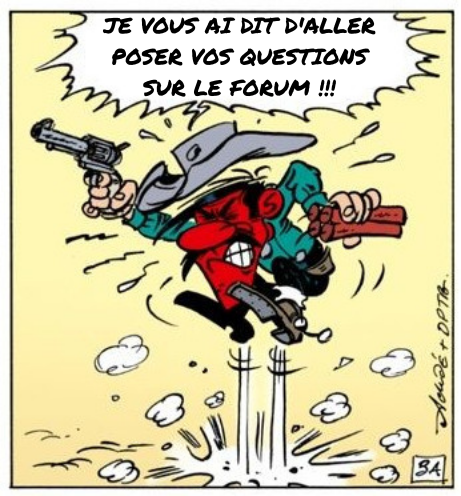
\includegraphics[width=0.7\linewidth]{../../../img/go_forum}
\end{center}
\label{go_forum}
\caption{J'pète les plombs}
\end{figure}}

\newcommand{\reponse}[4][1]
{\noindent
\parbox{\textwidth}{
\rule{\linewidth}{.5pt}\\
\textbf{Question\ifthenelse{#1>1}{s}{} \multido{}{#1}{%
\refstepcounter{num_rep}\ref{q\the\value{num_rep}} }:} ~\ \\
\ifdef{\public}{#3 \ifthenelse{#2>0}{~\ \\ 	\feuilleDR{#2}}}{#4}
}}

\newcommand{\cor}
{\refstepcounter{num_cor}
\noindent
\rule{\linewidth}{.5pt}
\textbf{Question \arabic{num_cor}:} \\
}

\newcommand{\finsujet}
{
    \begin{center}
    \Large{FIN}
    \end{center}

    \cleardoublepage

    \ifdef{\public}{\pagestyle{docreponse}}{\pagestyle{correction}}

    \ifdef{\public}{
        \begin{tikzpicture} 
            \draw (0,0) rectangle (2,2);
            \draw (0,0) -- (2,2);
            \draw (1.5,0.5) node {\large 20};
            \draw (2.5,0) rectangle (16,2);
            \draw (4.5,1.7) node {\large Commentaires:};
        \end{tikzpicture}
    }
    ~\ \\
}


%\newcommand{\repcarre}[2]
%{
%~\ \\
%\begin{tikzpicture}
%\draw [fill=white] (0,0) rectangle +(\linewidth,#1);
%\node[align=left] at (1.1,#2-0.3) {\textbf{Question #1:}};
%\end{tikzpicture}
%}

\newcommand{\titre}[1]
{\begin{center}
\cadre{0.8}{\huge #1} 
\end{center}
}


%Définition des torseurs :
\newcommand{\torseur}[2]{\left\{\mathcal{#1}_{#2} \right\}}
\newcommand{\torseurh}[3]{\left\{\genfrac{}{}{0pt}{0}{#1}{#2}\right\}_{#3}}
\newcommand{\torseurv}[8]{\left\{
\begin{matrix}
#1 & #4 \\ #2 & #5 \\ #3 &#6
\end{matrix}
\right\}_{{#7},{#8}}}

%Définition des torseurs :
%\newcommand{\torseur}[2]{\left \{\mbox{\relsize{2}{$\mathcal {#1}$}\relsize{-2}}\phantom{}_{\mbox{\scriptsize $#2$}} \right \}}
%\newcommand{\torseurh}[3]{\left\{\genfrac{}{}{0pt}{0}{#1}{#2}\right\}_{#3}}
%\newcommand{\torseurv}[8]{
%\left\{\begin{array}{@{}c|c@{}} #1 & #4 \\ #2 & #5 \\ #3 & #6 \end{array} \right\}_{#7,#8}
%}
\newcommand{\derivee}[2]{\left.\dfrac{\d #1}{\d t}\right|_{#2}}
\newcommand{\tripleint}{\int\!\!\!\!\!\int\!\!\!\!\!\int}

% Notation cinématique et statique
\newcommand{\cinematique}[2]{\mbox{#1}/\mbox{#2}}
\newcommand{\statique}[2]{\mbox{#1}\rightarrow\mbox{#2}}
\newcommand{\moment}[3]{\vv {#1}_{\scriptsize{#3}}(#2)}
\newcommand{\resultante}[2]{\vv {#1}_{\scriptsize{#2}}}


%Commande de base
\newcommand{\jo}{\left(j\omega\right)} % j \omega dans l'analyse fréquentielle
\newcommand{\tl}{\xrightarrow{\mathcal{L}}} % transformée de laplace sur fleche
\newcommand{\tli}{\xrightarrow{\mathcal{L}^{-1}}} % transformée inverse de laplace sur fleche
\renewcommand{\d}[1][]{\mathrm{d#1}}
\newcommand{\dd}[1][]{\mathrm{d#1}}
\newcommand{\vect}[2]{{#1}\wedge{#2}}
\newcommand{\base}[3]{(\vec #1,\vec #2,\vec #3)}
\newcommand{\vectbase}[4]{{\vphantom{\left| \begin{matrix}
#1\\#2\\#3 \end{matrix} \right|}}_{#4}{\left| \begin{matrix}
#1\\#2\\#3 \end{matrix} \right.}}
%Pour avoir les paragraphes sous la forme I, II, III
\renewcommand{\thesection}{\Roman{section}}
\setcounter{secnumdepth}{3}
\renewcommand{\Frlabelitemii}{$\bullet$}

% En tête et pied de page
\lhead{\nom}
\rhead{
\includegraphics[width=2cm]{../../../img/logo}}
\lfoot{\auteurun,\ \auteurdeux}
\cfoot{Page \thepage}

\fancypagestyle{docreponse}{%
  \fancyhf{}
  \fancyhead[LO]{NOM Prénom: .............................}
  \rhead{
\includegraphics[width=2cm]{../../../img/logo}\hspace{2pt}}
  \ifdef{\auteurdeux}{\lfoot{\auteurun,\ \auteurdeux}}{\lfoot{\auteurun}}
  \rfoot{\nom}
  \lfoot{Document réponse}
  \cfoot{Page \thepage}
   }

\fancypagestyle{correction}{%
  \fancyhf{}
  \lhead{\colorbox{danger}{\begin{minipage}{0.65\paperwidth} \textcolor{white}{\textbf{Correction}} \end{minipage}} }
  \rhead{
\includegraphics[width=2cm]{../../../img/logo}}
  \lfoot{Renaud Costadoat, Françoise Puig}
  \rfoot{\colorbox{danger}{\begin{minipage}{0.4\paperwidth} \begin{flushright}\textcolor{white}{\textbf{Correction}}\end{flushright} \end{minipage}} }}

\fancypagestyle{correctioninfo}{%
  \fancyhf{}
  \lhead{\colorbox{danger}{\begin{minipage}{0.65\paperwidth} \textcolor{white}{\textbf{Correction}} \end{minipage}} }
  \rhead{
\includegraphics[width=2cm]{../../../img/logo}}
  \lfoot{Renaud Costadoat, Juliette Genzmer}
  \rfoot{\colorbox{danger}{\begin{minipage}{0.6\paperwidth} \begin{flushright}\textcolor{white}{\textbf{Correction}}\end{flushright} \end{minipage}} }}

\renewcommand{\footrulewidth}{0.4pt}

\usepackage{eso-pic}
\newcommand{\BackgroundPic}{%
\put(0,0){%
\parbox[b][\paperheight]{\paperwidth}{%
\vfill
\begin{center}
\hspace{0.5cm}\vspace{0.5cm}

\includegraphics[width=\paperwidth,height=\paperheight,%
keepaspectratio]{../../../img/fond3}%
\end{center}
\vfill
}}}

\newcommand{\BackgroundPicdeux}{%
\put(25,-30){%
\parbox[b][\paperheight]{\paperwidth}{%
\vfill
\begin{center}
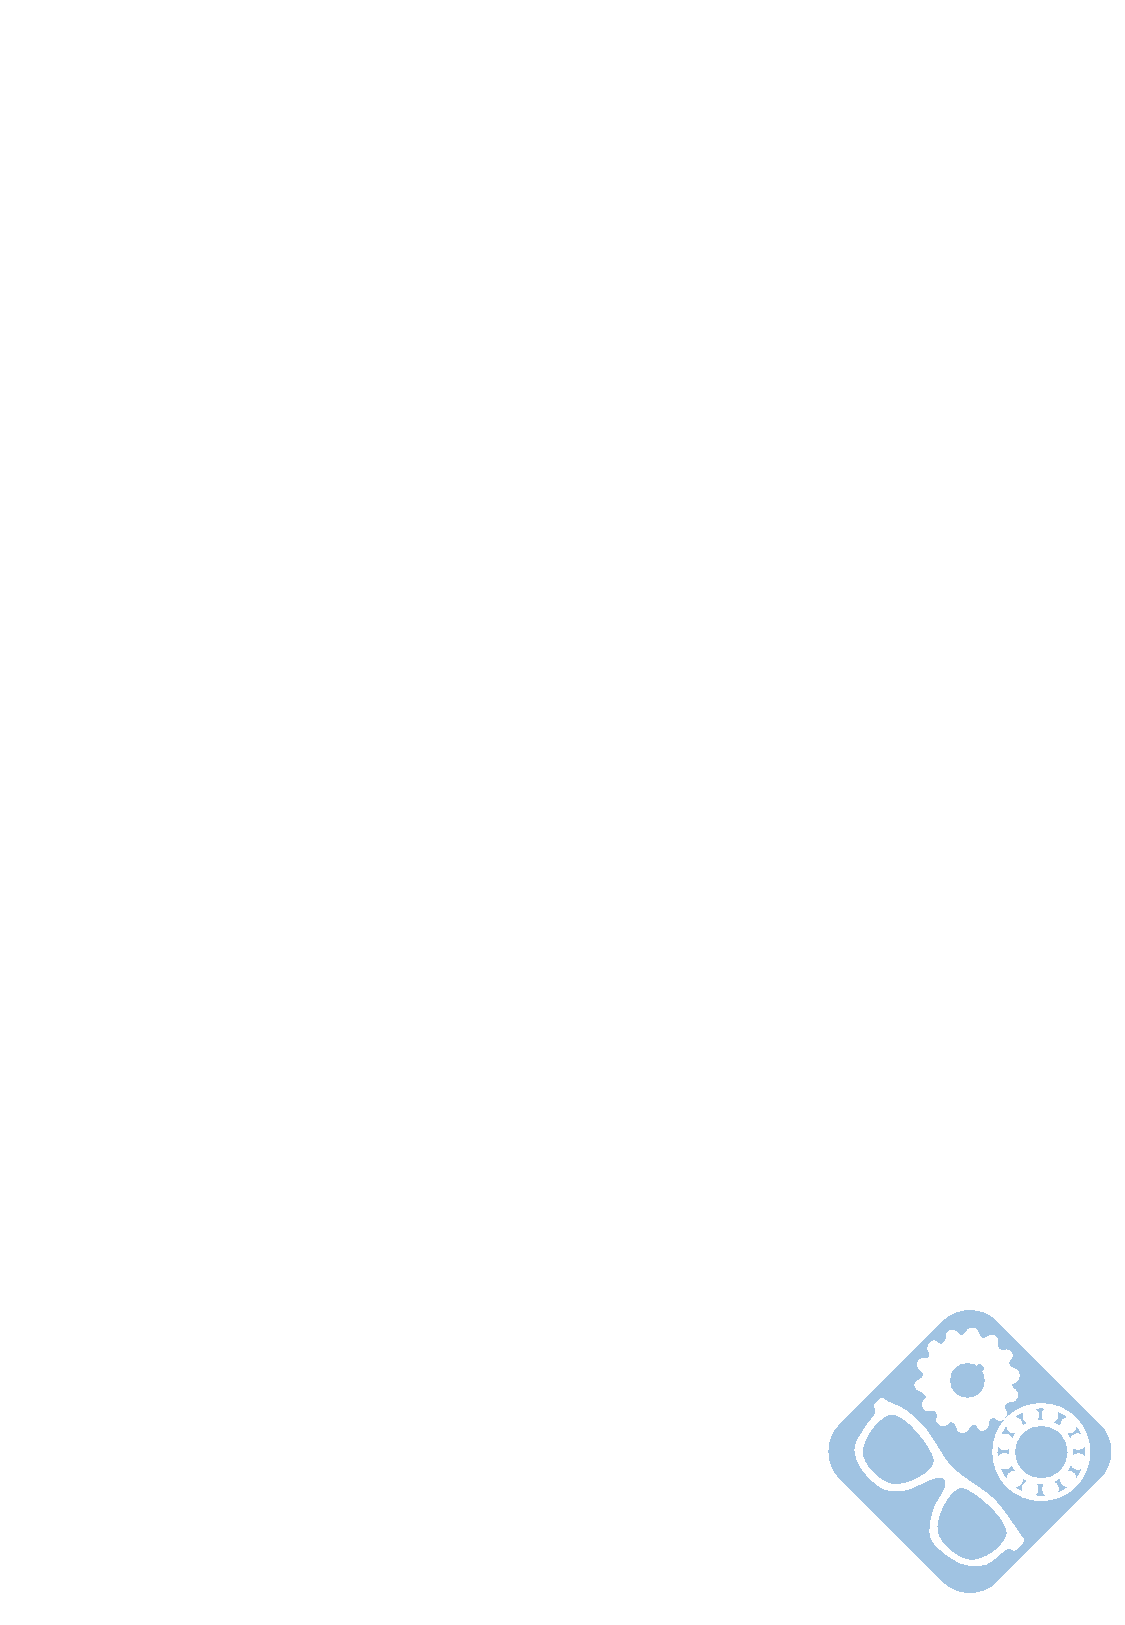
\includegraphics[width=\paperwidth,height=\paperheight,%
keepaspectratio]{../../../img/fond4}%
\end{center}
\vfill
}}}

\begin{document}

\pagestyle{empty}

\AddToShipoutPicture*{\BackgroundPic}


\includegraphics[width=2cm]{../../../img/logo}

\Huge{DS \numero - \sujet}

\vspace{1cm}

\ifdef{\prive}{\begin{center}\colorbox{danger}{\Huge{Avec Correction}}\end{center}}{}

\begin{center}
\centering\huge{PTSI}
\end{center}

\vspace{2cm}


\begin{center}
\centering\Large{\jour}
\end{center}

\vspace{2cm}

\normalsize

\tableofcontents

\newpage

\AddToShipoutPicture{\BackgroundPicdeux}

\pagestyle{fancy}

\begin{center}
\Huge \sujet
\end{center}


\normalsize


\section{Mise en situation}

La Société GBMA est une PME spécialisée dans la recherche, la conception, la fabrication, l'installation et la maintenance de matériels d'embouteillage semi automatiques ou automatiques. Parmi ces matériels, l'entreprise fabrique en petite série des boucheuses museleuses entièrement mécaniques et gérées par un automate programmable. 

Ces machines assurent :
\begin{itemize}
 \item Le serrage et l'enfoncement du bouchon dans la bouteille,
 \item La distribution et la mise en place du muselet (Armature de fil de fer dont on coiffe le bouchon des bouteilles de champagne).
\end{itemize}

\begin{figure}[!h]
\begin{center}
	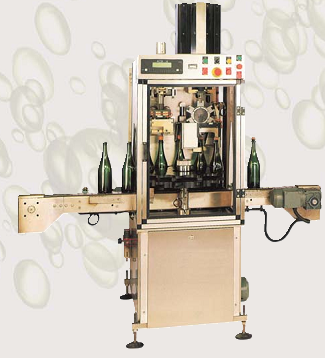
\includegraphics[width=0.4\linewidth]{img/fig01}
\end{center}
\caption{Boucheuse museleuse}
\label{fig01}
\end{figure} 

Tous les éléments de la machine qui risquent d'être en contact avec les bouteilles ou les bouchons sont en acier inoxydable. Le réglage de la cadence est réalisé par un potentiomètre sur le tableau de bord (800 à 2400 bouteilles par heure). Cette machine permet le traitement des demi-bouteilles, bouteilles et magnums de champagne. Elle est plus particulièrement destinée à équiper les petites exploitations viticoles.

\section{Description de la partie opérative (limitée au compresseur de bouchons)}

Une des fonctions que doit garantir la machine est de réduire le diamètre du bouchon en liège de 30 à 16 mm. Le bouchon peut ainsi être poussé à l'aide d'un poussoir dans le goulot d'une bouteille de champagne qui fait 18 mm de diamètre.

Pour réduire le diamètre des bouchons, on utilise un compresseur à bouchons (voir annexe 1). L'ouverture et la fermeture des 4 mors sont assurées par une came. Cette came est en liaison encastrement avec l'arbre principal de commande. Sur cet arbre, il y a d'autres cames permettant de garantir d'autres fonctions. Cet arbre est commandé par un moto-réducteur à courant continu (230V, 1050 tr/mn, 1200W).

L'arbre principal de commande tourne à fréquence de rotation constante. \textbf{Chaque fois qu'il fait un tour, une bouteille est bouchée et muselée}.

L'ensemble de l'étude portera principalement sur le compresseur à bouchons et la came de commande pour les parties cinématiques, statique et communication technique ainsi que sur la commande du moteur pour la seule partie automatique.

\section{Étude fonctionnelle}

Les bouteilles de champagnes, une fois dégorgées et dosées en liqueur (brut, sec ou demi-sec), sont bouchées puis muselées sur une machine automatique appelée boucheuse museleuse. On donne ci-dessous le diagramme des cas d'utilisation partiel de cette machine.

\begin{figure}[!h]
\begin{center}
	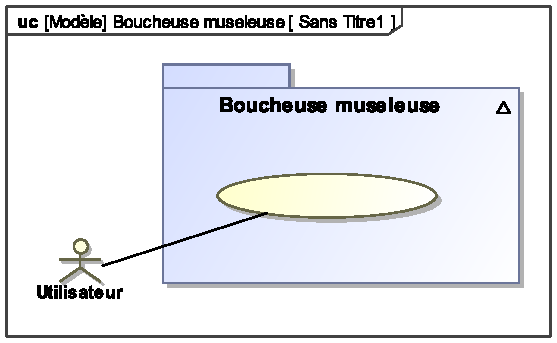
\includegraphics[width=0.4\linewidth]{img/fig02}
\end{center}
\caption{Diagramme des cas d'utilisation}
\label{fig02}
\end{figure} 

\question{Donner le cas d'utilisation correspondant à ce système.}

\begin{figure}[!h]
\begin{center}
	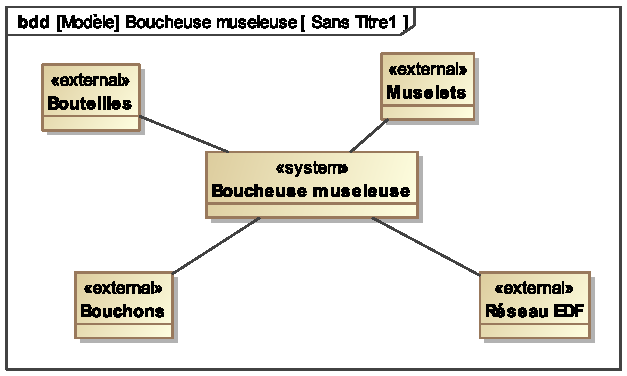
\includegraphics[width=0.4\linewidth]{img/fig03}
\end{center}
\caption{Diagramme de contexte}
\label{fig03}
\end{figure} 

\question{Donner au moins deux autres éléments du milieu extérieur au système non présents dans la description de la figure \ref{fig03}.}

\question{Justifier le fait que les éléments du diagramme de contexte ne se retrouvent pas tous dans le diagramme des cas d'utilisation.}

\section{Étude cinématique}

L'objectif de cette étude est de déterminer certains éléments permettant de valider les choix de solutions retenues pour les guidages en rotation du galet et en translation du coulisseau.

Pour ce qui suit, la machine est réglée à sa cadence maximale, c'est à dire 2400 bouteilles par heure. L'arbre principal de commande tourne à fréquence constante.

\question{Calculer la vitesse de rotation $\dot{\theta}$ de l'arbre principal. Donner le résultat en fonction de $\pi$ et en $rad.s^{-1}$.}

\question{Un galet de diamètre 30 mm est en liaison pivot avec le coulisseau (1) qui commande le serrage des mors (voir annexe 1). La came, dont le profil est donné à l'échelle 1 en annexe 2, agit sur ce galet. Après avoir relevé toutes les dimensions utiles sur l'annexe 2, tracer la courbe donnant la loi de mouvement du centre du galet (O') en fonction de l'angle de rotation de la came.}

\question{Tracer en rouge, sur le dessin du document réponse, les directions de : $\overrightarrow{V_{I\in 1/0}}$, $\overrightarrow{V_{I\in 2/0}}$ et $\overrightarrow{V_{I\in 2/1}}$, en remarquant que le mors (5) \textbf{est fixe par rapport au bâti}.}

\begin{figure}[!h]
\begin{center}
	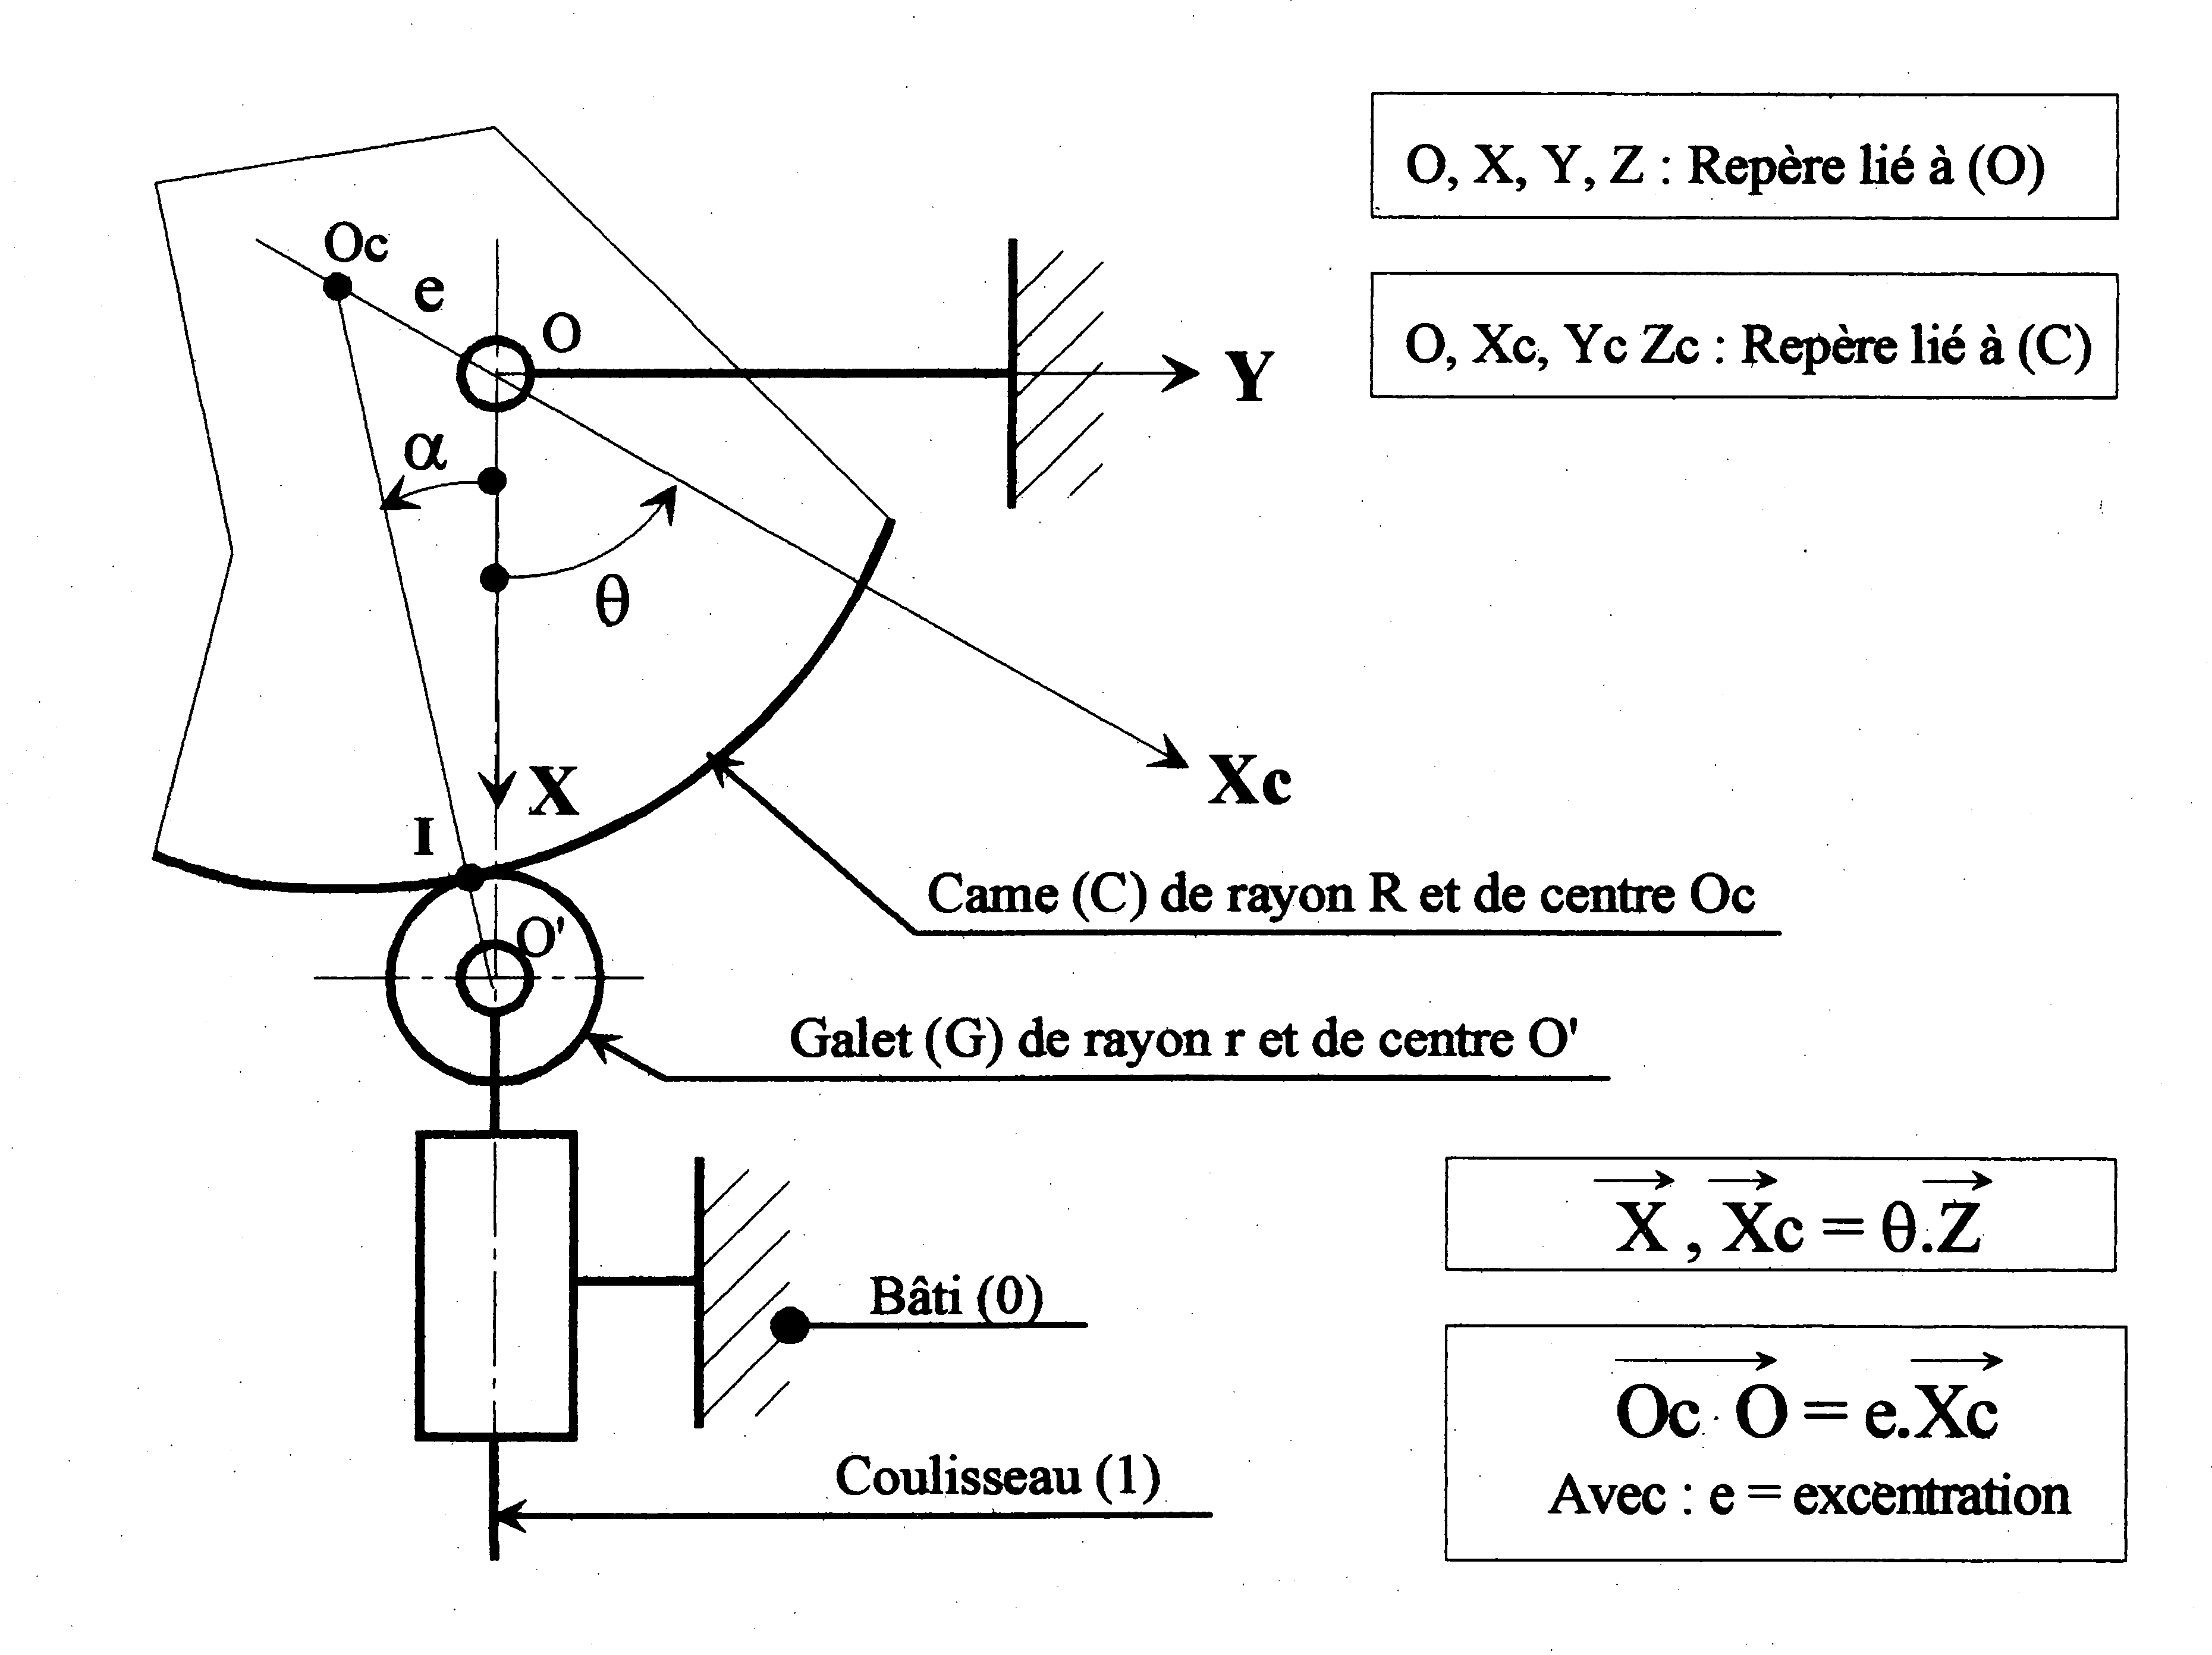
\includegraphics[width=0.8\linewidth]{img/fig04}
\end{center}
\caption{Modèle cinématique}
\label{fig04}
\end{figure} 

\question{On pose : $\overrightarrow{V_{I\in 1/0}}.\overrightarrow{x}=V$. Calculer, en fonction de $V$ et des paramètres géométriques, les vitesses $\overrightarrow{V_{I\in 1/0}}$, $\overrightarrow{V_{I\in 2/0}}$ et $\overrightarrow{V_{I\in 2/1}}$. (L'angle entre $\overrightarrow{x}$ et $\overrightarrow{x_2}$ est à lire sur l'annexe 1.)}

~\

Pour : $60\degree \leq \theta \leq 240\degree$, le profil de la came est une portion de cercle de centre $O_c$ et de rayon $R$. La came tourne autour du point $O$. Le galet (G) de rayon $r$ et de centre $O'$ roule sans glisser sur le profil de la came au point $I$. Le galet est en liaison pivot d'axe  par rapport au coulisseau (1).

\question{\begin{enumerate}
 \item Soit $\overrightarrow{O_CI}=R.\overrightarrow{x_i}$, exprimer le vecteur $\overrightarrow{x_i}$ dans la base ($\overrightarrow{X},\overrightarrow{Y},\overrightarrow{Z}$),
 \item Exprimer l'angle $\alpha$ en fonction de : $e$, $\theta$, $R$ et $r$,
 \item Déterminer la vitesse du point $I$ appartenant à la came (C) par rapport au bâti (0), dans la base $(\overrightarrow{x},\overrightarrow{y},\overrightarrow{z})$ en fonction de : $e$, $\theta$, $\dot{\theta}$, $R$ et $r$,
 \item Déterminer le torseur cinématique du mouvement du galet (G) par rapport au bâti (0), dans la base ($\overrightarrow{x},\overrightarrow{y},\overrightarrow{z}$) et au point O' en fonction de $e$, $\theta$, $\dot{\theta}$, $R$ et $r$.
\end{enumerate}}

\section{Étude statique}

On se propose avec cette étude de déterminer les efforts qui s'exercent sur les mors en fin de phase de compression du bouchon ($\theta= 240\degree - \epsilon$) afin d'être en mesure de dimensionner certains éléments du compresseur.

Pour simplifier le problème on limitera l'étude au seul mors (2) et on fera les hypothèses suivantes :
\begin{itemize}
 \item L'étude est assimilée à un problème de statique plane,
 \item Répartition uniforme des pressions de contact entre les différents solides,
 \item Le poids des mors est négligeable,
 \item Le mors glisse sur le coulisseau (1) et sur les mors (3) et (5),
 \item Le mors ne glisse pas par rapport au bouchon,
 \item Le coefficient de frottement entre les pièces (1), (2), (3), (4) et (5) est f.
\end{itemize}

Notation de l'action mécanique de $S_i \rightarrow S_j$ au point P :

\begin{center}
$\left\{T_{S_i \rightarrow S_j}\right\}=\left\{
\begin{array}{cc}X_{Pij} & L_{Pij}  \\
Y_{Pij} & M_{Pij}  \\
Z_{Pij} & N_{Pij}
\end{array}
\right\}_{P,R}$
\end{center}

\question{Calculer la norme $\|\overrightarrow{E_{R\rightarrow 2}}\|$ de l'effort du ressort (R) sur le mors (2) si la raideur $k$ du ressort est de $4N.mm^{-1}$ et si sa longueur libre (état non comprimé) est de $50mm$. En fin de phase de compression, on peut vérifier sur l'annexe 1 (en tenant compte de l'échelle) que le ressort mesure $30mm$.}

~\

Sur le document réponse, on a isolé le mors (2) à l'échelle 2.

On modélise :
\begin{itemize}
 \item L'action de (1) sur (2) par un glisseur dont le support passe par A,
 \item L'action de (3) sur (2) par un glisseur dont le support passe par B,
 \item L'action de (5) sur (2) par un glisseur dont le support passe par C,
 \item L'action du bouchon sur (2) par un glisseur dont le support passe par D,
 \item L'action du ressort sur (2) par un glisseur dont le support passe par E.
\end{itemize}

On appelle $F=\|\overrightarrow{F}\|$ avec $\overrightarrow{F}$ résultante de l'action du bouchon sur (2). $\overrightarrow{F}$ est donnée sur la figure du document réponse. Une étude expérimentale a permis de la connaître en sens et en intensité.

\question{Tracer en rouge sur la figure les différentes actions mécaniques qui s'exercent sur le mors (2). Indiquer clairement le sens et l'angle de frottement $\varphi$ si nécessaire.}

~\

On rappelle que l'on est en phase de fin de compression, donc que le mors (2) glisse par rapport aux mors (3) et (5) et par rapport au coulisseau (1). On rappelle d'autre part que le mors (5) est fixe.

\question{Ecrire les 3 équations scalaires traduisant l'équilibre du mors (2) si l'on néglige l'action du ressort. Ces équations seront données dans la base ($\overrightarrow{X_2},\overrightarrow{Y_2},\overrightarrow{Z_2}$) liée au mors (2), en fonction de $F$, $f$, des données géométriques et des composantes en valeur absolue des actions mécaniques $X_{A12}$, $X_{B32}$ et $Y_{C52}$. L'équation de moment sera écrite au point H (voir le document réponse).}

~\

La résolution des trois équations scalaires a permis de déterminer les différentes inconnues statiques de la question précédente. On obtient : $\overrightarrow{A_{1\rightarrow2}}=13585.\overrightarrow{x_2}-679.\overrightarrow{y_2}$ (en newton).

Par ailleurs un calcul de statique appliqué au mors (3) donne :

$\overrightarrow{F_{3\rightarrow1}}.\overrightarrow{x}=-10000N$.

\question{En négligeant les frottements du coulisseau (1) par rapport au bâti (0), calculer numériquement $\|\overrightarrow{R_{C\rightarrow G}}\|$ la norme de la résultante de l'action de la came (C) sur le galet (G) en fin de phase de compression du bouchon.}

\section{Étude de l'asservissement du moteur}

L'objectif de cette étude est de vérifier que le moteur utilisé permet d'obtenir la cadence de 2400 bouteilles / heure.

Hypothèse : On se place dans le cas d'un système linéaire, continu et invariant.

Modélisation du moteur : Le moteur qui entraîne l'arbre principal est équipé d'un moteur à courant continu. Le modèle de connaissance de cet actionneur, si on néglige l'inductance et les différents frottements, permet d'écrire les équations électromécaniques suivantes :

$\left\{\begin{array}{l}
e(t)=u(t)-R.i(t)=K_e.\omega(t) \\
C_m(t)=Kt.i(t)=J.\frac{d\omega(t)}{dt}
\end{array}\right.$

Avec: 
\begin{itemize}
 \item $u(t)$: Tension d'entrée en $V$,
 \item $\omega(t)$: fréquence angulaire de l'arbre du moteur en $rad.s^{-1}$,
 \item $e(t)$: force électromotrice en $V$,
 \item $R$: résistance de l'induit en $\Omega$,
 \item $K_e$: constante de force électromotrice $V.rad^{-1}.s$,
 \item $K_c$: constante de couple en $N.m.A^{-1}$,
 \item $C_m(t)$: couple électromécanique délivré par le moteur en $N.m$,
 \item $J$: moment d'inertie équivalent rapporté à l'arbre de sortie en $kg.m^2$.
\end{itemize}

\question{Écrire les 4 équations ci-dessus dans le domaine de Laplace si toutes les conditions initiales sont nulles.}

\question{En fonction des résultats trouvés à la question précédente, compléter le schéma blocs proposé sur le document réponse.}

\question{Calculer la fonction de transfert $H(p)=\frac{\Omega(p)}{U(p)}$ de ce moteur. Donner la réponse sous la forme canonique.}

\newpage

Par une expérimentation du moteur en charge, on a relevé les diagrammes de Bode (Modèle de comportement), ils sont présentés ci-dessous.

\begin{figure}[!h]
\begin{center}
	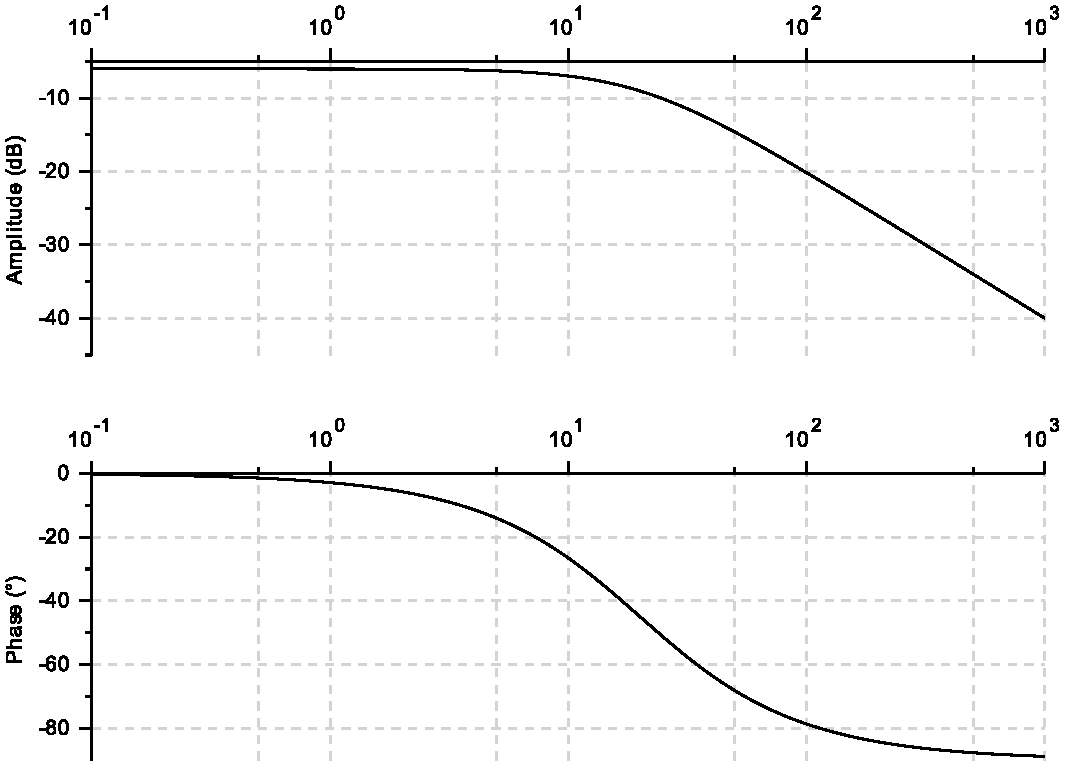
\includegraphics[width=0.7\linewidth]{img/fig05a}
\end{center}
\caption{Diagrammes de Bode du moteur}
\label{fig05a}
\end{figure} 

\question{Déterminer l'ordre du système ainsi que la constante de temps $\tau$ et le gain statique $K_s$. Justifier la réponse. Écrire numériquement la fonction de transfert du moteur sous la forme canonique.}

~\

Les caractéristiques techniques du moteur annoncées par le constructeur sont:\\
$R=3,4\Omega$ et $K_t=0,85N.m.A^{-1}$.

\question{Calculer la valeur de $K_e$ ($V.rad^{-1}.s$) et celle de $J$ ($kg.m^2$).}

\question{Tracer la réponse temporelle de ce moteur s'il est soumis à un échelon de tension$U_0=220V$. Indiquer la pente à l'origine et le temps de réponse à 5\%.}

~\

Pour la suite, on prendra pour la fonction de transfert de ce moteur :
\begin{center}
$H(p)=\frac{0,5}{1+0,05.p}$
\end{center}

\subsection{Asservissement en vitesse de l'arbre de sortie du moteur}

Pour assurer l'asservissement de la vitesse de rotation de l'arbre de sortie du moteur (donc de l'arbre principal), on associe à l'actionneur un variateur modélisé par un amplificateur pur de gain $K_a$ réglable.

\begin{figure}[!h]
\begin{center}
	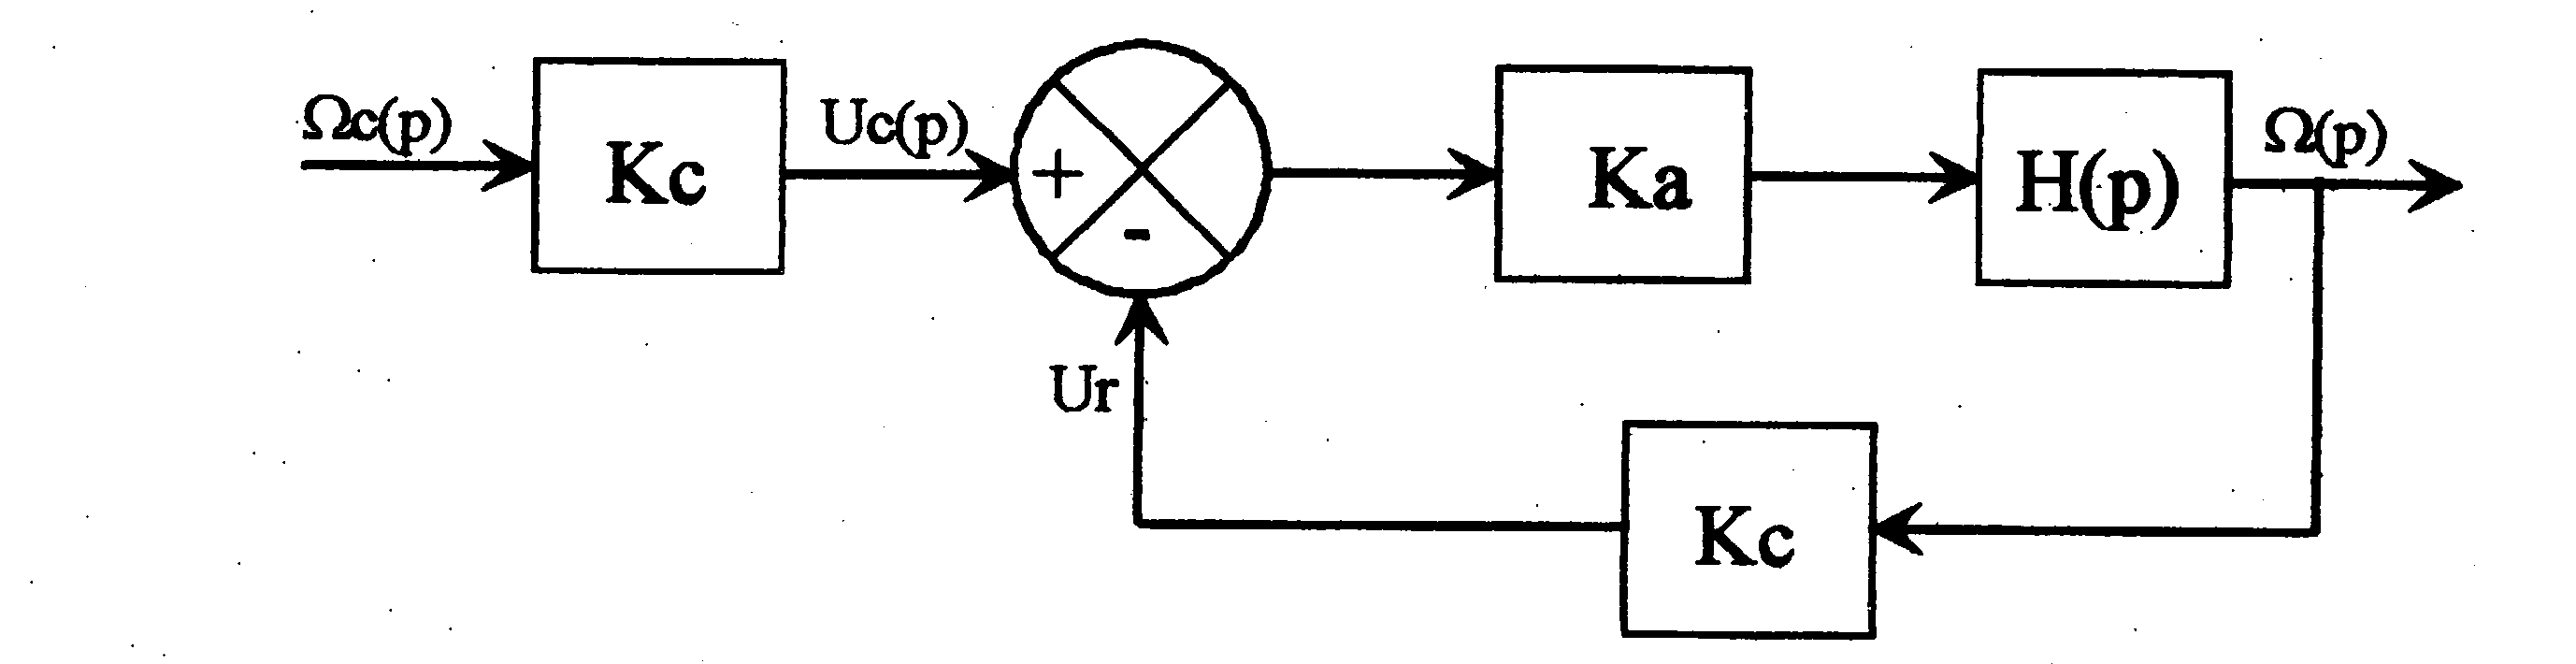
\includegraphics[width=0.7\linewidth]{img/fig05b}
\end{center}
\caption{Modèle de l'asservissement}
\label{fig05b}
\end{figure} 

On a placé un capteur de vitesse angulaire en bout de l'arbre de sortie de gain $K_c=0,06V.rad^{-1}.s$.
 
\newpage

\question{Calculer la fonction de transfert $F(p)=\frac{\Omega(p)}{\Omega_c(p)}$ de ce système en boucle fermée en fonction de $K_a$ et des valeurs numériques.}

\question{Tracer la réponse temporelle de cet asservissement s'il est soumis à un échelon $\Omega_c=100rad.s^{-1}$ et si $K_a=800$. En déduire l'erreur statique $\epsilon_s$ (écart entre la valeur de consigne et la valeur réelle).}

\question{Quelle valeur faudrait-il donner à $K_a$ si on souhaite une erreur $\epsilon_s \leq 2\%$ ?}

\section{Étude de fabrication et de construction}

\question{Donner un procédé de fabrication permettant de fabriquer la pièce suivante, la série de fabrication sera de 1000 pièces.}

 \begin{figure}[!h]
\begin{center}
	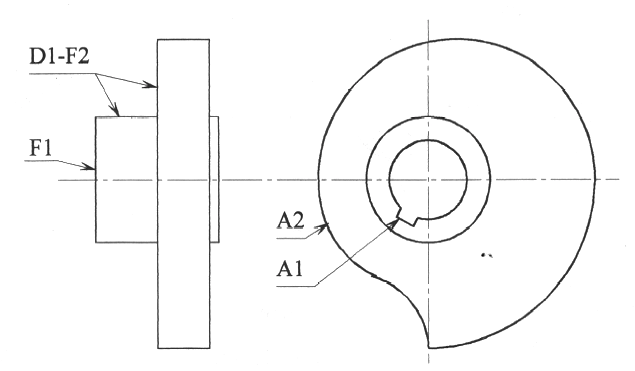
\includegraphics[width=0.6\linewidth]{img/fig06}
\end{center}
\caption{Galet excentrique}
\label{fig06}
\end{figure} 

\question{Donner la désignation des pièces repérées A, B et C (voir calque réponse)}

\question{Proposer et justifier un procédé de fabrication pour le carter}

\question{Proposer un modèle de liaison entre l'arbre principal (103) et le bâti (100+101+110+...) (voir annexe 3):
\begin{enumerate}
 \item Au niveau du roulement (102),
 \item Au niveau du roulement (111).
\end{enumerate}}

\question{Réaliser le schéma d'architecture limité au guidage de l'arbre principal (103) avec le bâti (100).

Donner le nom de la liaison équivalente entre l'arbre (103) et le bâti (100).}

\question{Indiquer un ajustement possible entre la came (106) et l'arbre principal (103).}

L'étude statique a montré que l'action du galet (120) sur la came (107) est très importante. L'arbre principal (103) va donc fléchir anormalement. Afin de remédier à cet inconvénient, on ajoute un roulement à billes (105) dans une zone proche des efforts à encaisser. Ce roulement est arrêté en translation par rapport à l'arbre (103) et est en liaison pivot glissant avec le support du compresseur (122).

Pour des raisons de simplicité de fabrication et de moindre coût, on impose :
\begin{itemize}
 \item Que le diamètre de l'arbre principal ne doit être ni augmenté ni diminué,
 \item Que le compresseur doit pouvoir être démonté très facilement (indépendamment de l'arbre principal et de ses pièces montées dessus),
 \item Que le support (122) doit être obtenu par usinage à partir d'un laminé marchand de nuance S235 (acier de construction d'usage général, ayant une limite minimale d'élasticité de 235 MPa) et de section 150 x 25 x L (L étant fonction de votre conception)
\end{itemize}

\question{Compléter le calque par une solution montrant la liaison du roulement (105) par rapport à l'arbre (103) et au support (122). Indiquer tous les ajustements permettant de valider votre solution.}

~\

Un axe devra traverser le galet (120) et sera encastré dans la pièce (123), on donne la solution de cet encastrement :

\begin{figure}[!h]
\begin{center}
	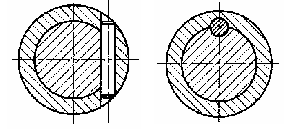
\includegraphics[width=0.6\linewidth]{img/fig08}
\end{center}
\caption{Montage goupille \og entre cuir et chair \fg}
\label{fig08}
\end{figure} 

\question{Intégrer cette solution sur le calque réponse, en vue A-A et coupe B-B.}

Remarque : le coulisseau repéré ici (123) était repéré (1) dans les parties précédentes pour une simplification d'écriture.

\subsection{Étude de spécifications}

Soit le modèle de spécifications suivantes:

\begin{figure}[!h]
\begin{center}
	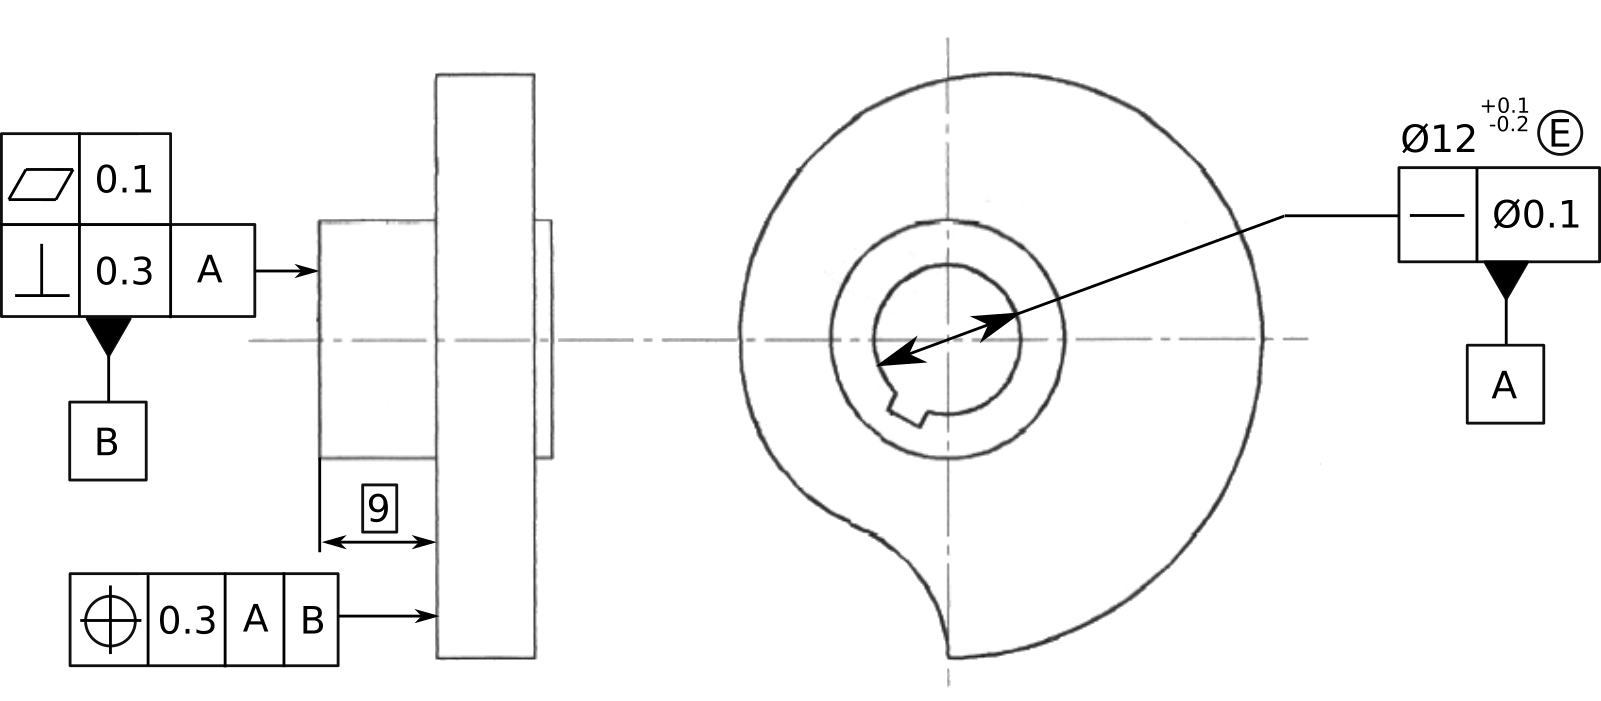
\includegraphics[width=0.6\linewidth]{img/fig06_2}
\end{center}
\caption{Modèle de spécifications du galet excentrique}
\label{fig08}
\end{figure} 

\question{Expliciter la spécification 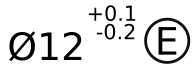
\includegraphics[width=2cm]{img/specif_5} sur une page libre ou sur un tableau GPS.}

\question{Expliciter la spécification 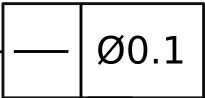
\includegraphics[width=2cm]{img/specif_1} sur une page libre ou sur un tableau GPS.}

\question{Expliciter la spécification 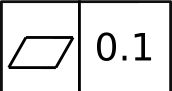
\includegraphics[width=2cm]{img/specif_2} sur une page libre ou sur un tableau GPS.}

\question{Expliciter la spécification 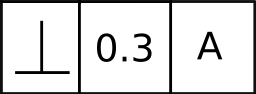
\includegraphics[width=2cm]{img/specif_3} sur une page libre ou sur un tableau GPS.}

\question{Expliciter la spécification 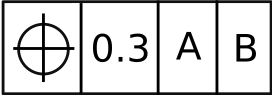
\includegraphics[width=2cm]{img/specif_4} sur une page libre ou sur un tableau GPS.}

\section{Étude combinatoire}

Le cogite est un système de compensation de gîte présent sur des porte-avions tels que le porte-avions Clémenceau ou le porte-avions Charles de Gaulle.

La partie opérative du cogite est constituée de 12 trains de 12 chariots à quatre roues (masse d'un train : $Mt = 22 tonnes$, inertie des roues négligeable) pouvant se déplacer sur la largeur du navire ($\pm 16m$)
Chaque train est entraîné par un moteur électrique relié à un réducteur, lui même accouplé à une poulie, tournant à une vitesse $\omega_p$, entraînant le câble. Deux freins permettent l'arrêt des masses.

\begin{figure}[!h]
\begin{center}
	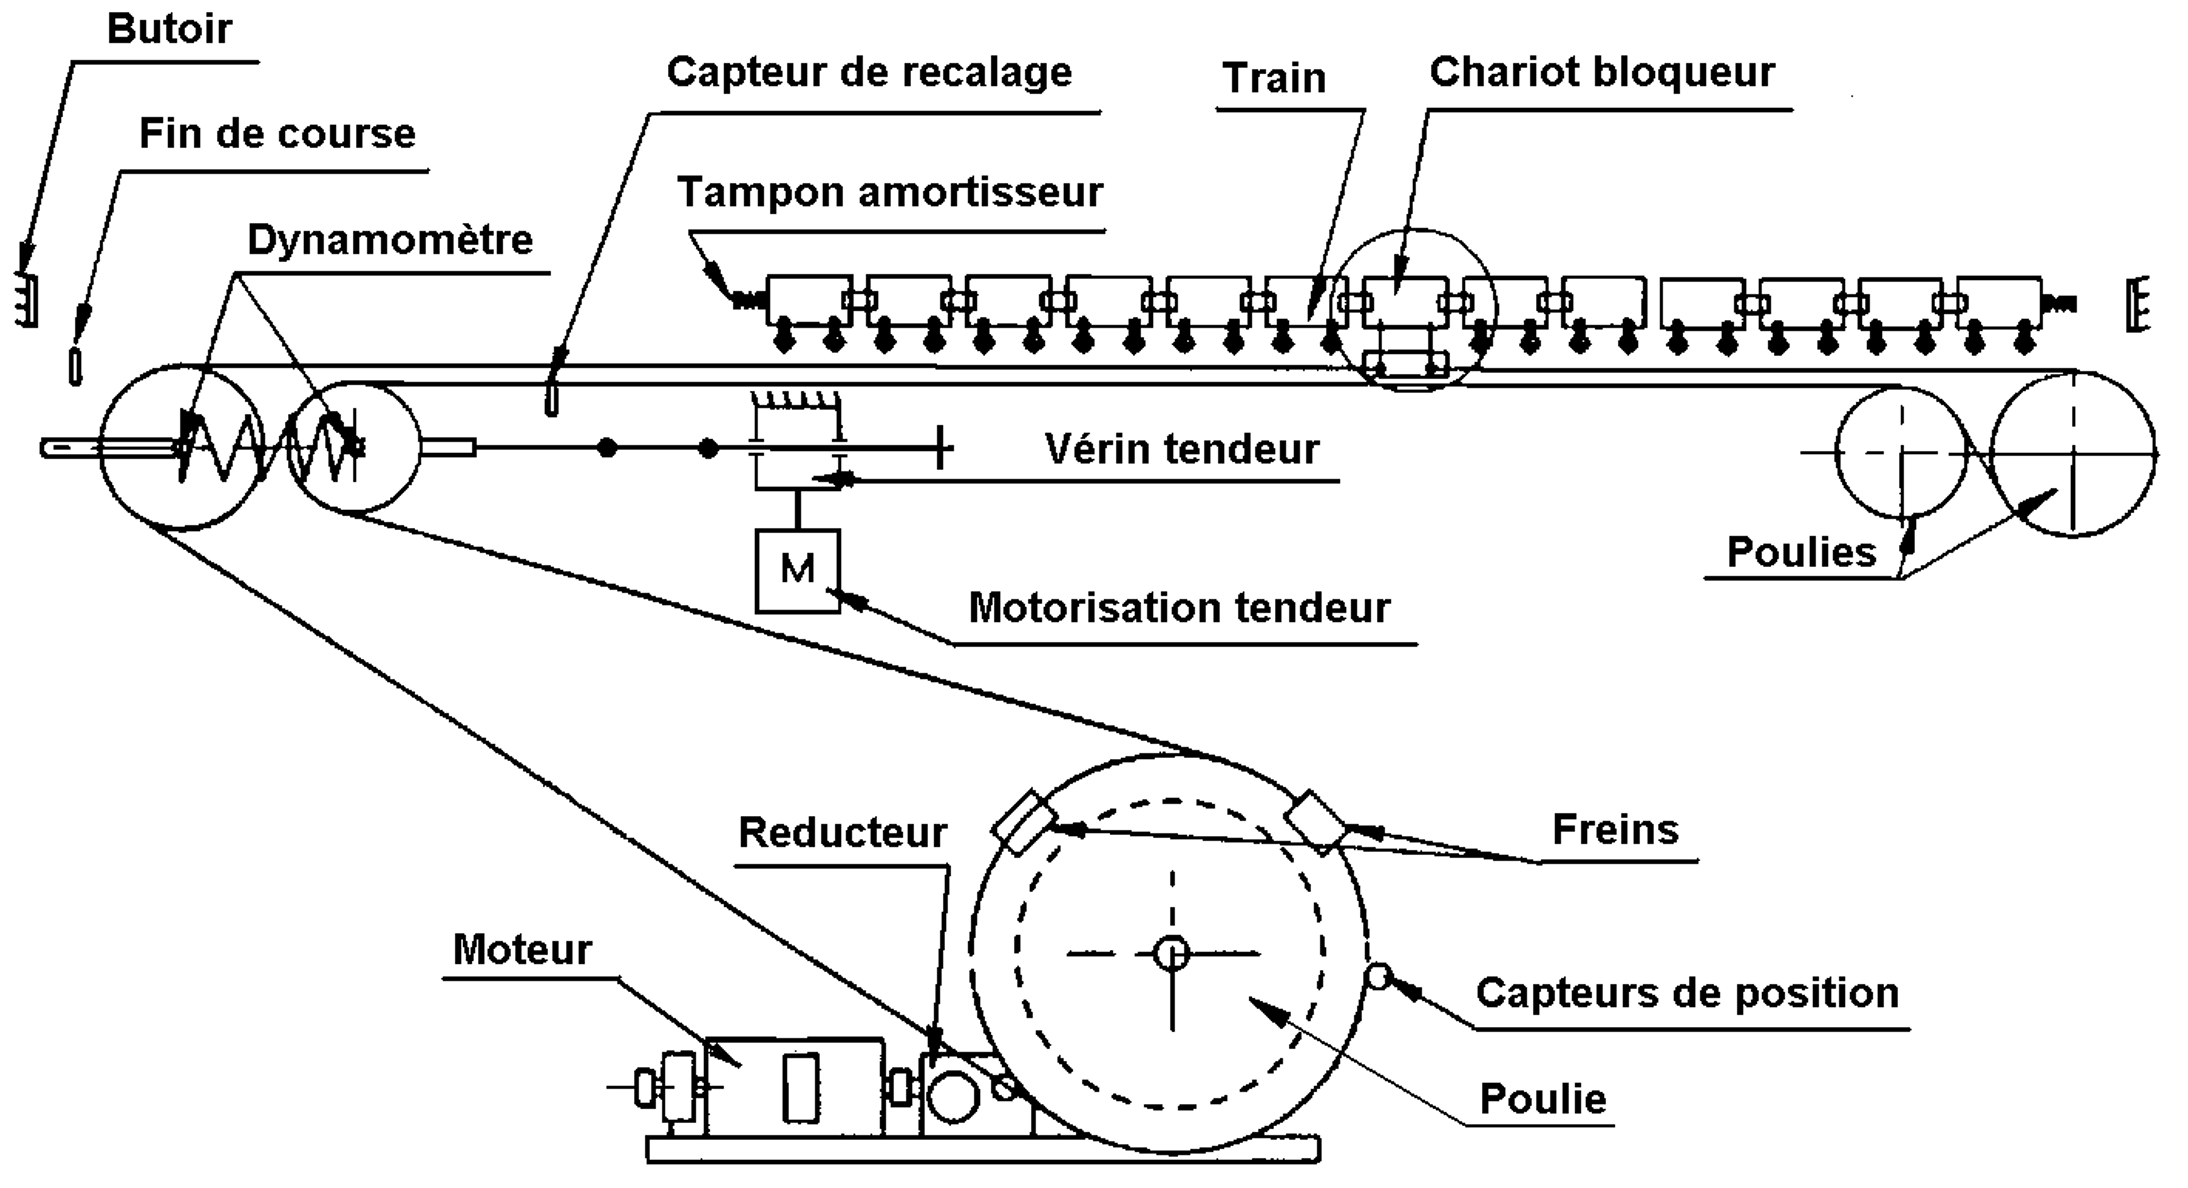
\includegraphics[width=0.8\linewidth]{img/fig09}
\end{center}
\caption{Système de transport de bouteilles}
\label{fig09}
\end{figure} 

\begin{table}[!h]
\begin{tabular}{|m{3.5cm}|m{5.5cm}|m{7cm}|}
\hline
Actionneurs	& Capteurs& Effecteurs \\
\hline
\textbf{Moteur principal :} Convertit une énergie électrique en énergie mécanique

\textbf{Motorisation tendeur :} Convertit une énergie électrique ou hydraulique (on ne sait pas) en énergie mécanique.
& 
\textbf{Capteur de position :} Donne indirectement la position du chariot bloqueur en mesurant la position angulaire de la poulie

\textbf{Dynamomètre :} Mesure l'effort de tension

\textbf{Fin de course :} Signale que le train atteint la position extrême (TOR)
Capteur de recalage : Permet sans doute de corriger l'information fournie par le capteur de position en prenant en compte les modifications dues au réglage de la tension et au glissement du câble sur la poulie.
&
\textbf{Chariot bloqueur et Train :} Agissent directement sur la matière d'\oe uvre (répartition des masses du navire...)
Les effecteurs secondaires agissent sur la masse mobile.

\textbf{Réducteur, Poulie, Câble :} Transformation du mouvement (rotation en translation, augmentation du couple donc de l'effort de traction).

\textbf{Frein :} Bloque le train en position

\textbf{Tampon amortisseur, Butoir :} Arrêt du train en fin de course

\textbf{Vérin tendeur :} Réglage de la tension du câble (tension initiale, rattrapage de l'extension due à l'usure...) \\
\hline
\end{tabular}
\caption{Composants du système}
\label{tab01}
\end{table}

Afin de contrôler chaque 1/10 de tour d'une poulie, un ensemble de trois détecteurs lit 4 pistes angulaires adjacentes situées sur la poulie (noir = 1, blanc = 0) (cf. figure ci-dessous).

\begin{figure}[!h]
\begin{center}
	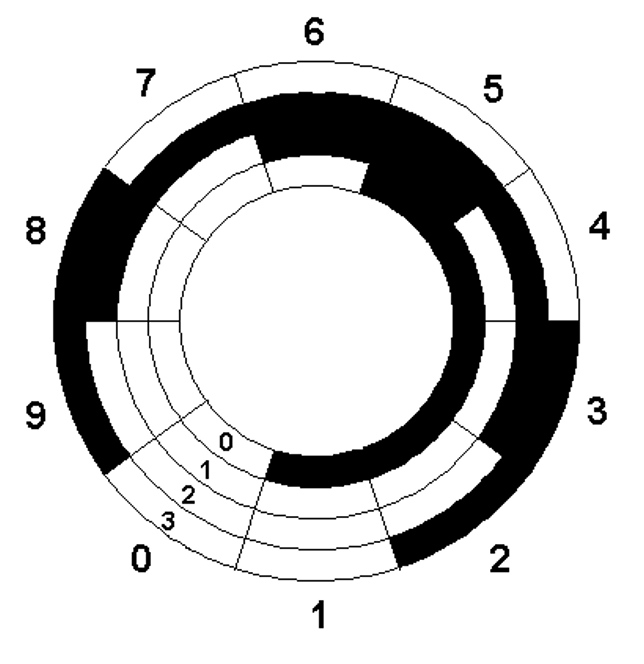
\includegraphics[width=0.3\linewidth]{img/fig10}
\end{center}
\vspace{-1cm}
\caption{Codeur}
\label{fig10}
\end{figure} 

Ces trois détecteurs : $A(a_0,a_1,a_2,a_3)$, $B(b_0,b_1,b_2,b_3)$ et $C(c_0,c_1,c_2,c_3)$ sont formés de quatre cellules photoélectriques.
						
Par exemple : $a_0$, $b_0$, $c_0$ lisent la \textbf{même} piste. La valeur des bits $d_i$ du détecteur de position $D(d_0,d_1,d_2,d_3)$ se construit à la \textbf{majorité} des valeurs des bits $a_i$, $b_i$ et $c_i$ des détecteurs A, B et C.
		
Ce système permet au calculateur de gérer les aléas de passage d'une position à une autre et de faciliter la maintenance du système.

En cas de désaccord sur un bit en position $i$, le bit $e_i$ d'un mot  $E(e_0,e_1,e_2,e_3)$ est placé à 1.

\question{Sachant que la poulie d'entraînement des câbles a un rayon de 0,795 m ($2\times \pi\times 0,795\simeq 5$), à combien de tours correspondent un déplacement d'un train de 32 m ? Quelle sera alors la précision de la mesure ?}

\question{Déterminer l'expression de $d_i=f(a_i,b_i,c_i)$ et de $e_i=g(a_i,b_i,c_i)$.}

\question{Proposer un schéma de câblage des $d_i$ avec des portes logiques NON, ET et OU.}

On désire afficher la valeur lue par D sur un pupitre indépendant du calculateur (en cas de dysfonctionnement de celui-ci). Pour cela, il est nécessaire de transcoder D en binaire naturel (soit K ce mot de 4 bits)

\question{Déterminer $K(k_0,k_1,k_2,k_3)$ en fonction de $D(d_0,d_1,d_2,d_3)$.}

\question{Écrire les fonctions de la manière la plus condensées possible en utilisant les fonctions logiques les plus appropriées : NON, ET, NON OU, NON ET, OU EXCLUSIF.}

~\

Pour permettre l'allumage d'une lampe témoin, on donne le schéma de câblage en technologie \og contacts électriques \fg suivant :

\begin{figure}[!h]
\begin{center}
	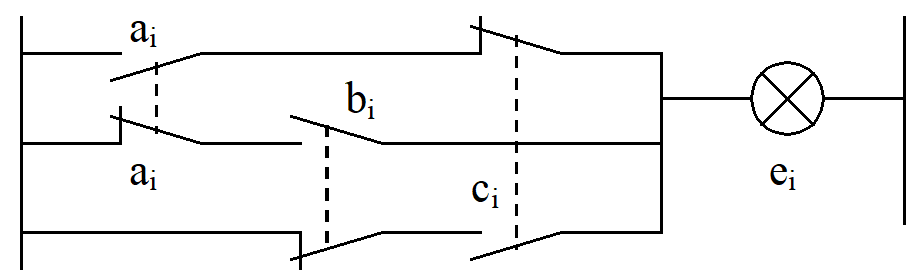
\includegraphics[width=0.5\linewidth]{img/fig11}
\end{center}
\caption{Schéma logique}
\label{fig11}
\end{figure} 

\question{Écrire pour l'exemple de la figure $e_i$ en fonction de $a_i$, $b_i$ et $c_i$.}

\question{Tracer le schéma logique correspondant à $k_1$.}

\begin{center}
----- FIN DU SUJET -----
\end{center}

\cleardoublepage


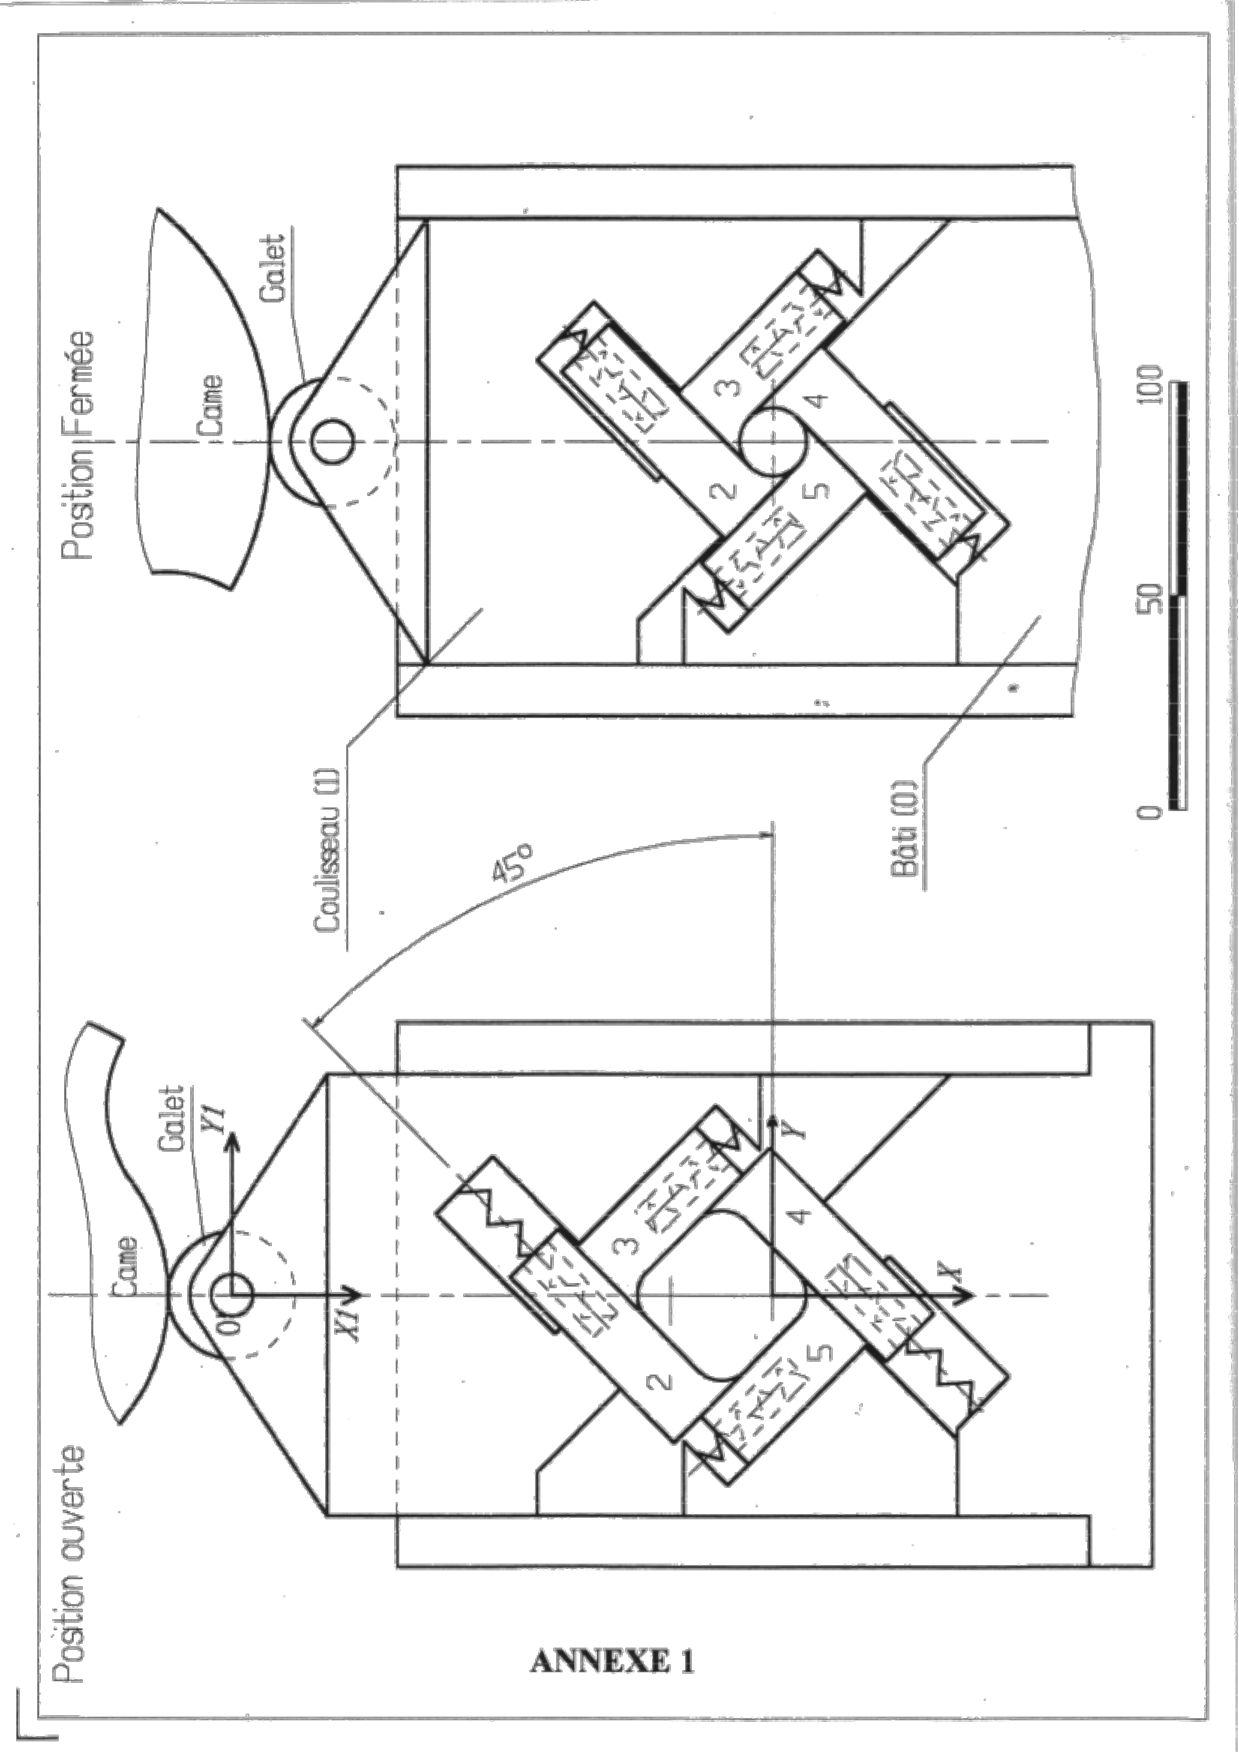
\includepdf[offset=0.5cm -1cm]{img/Annexe1.pdf}

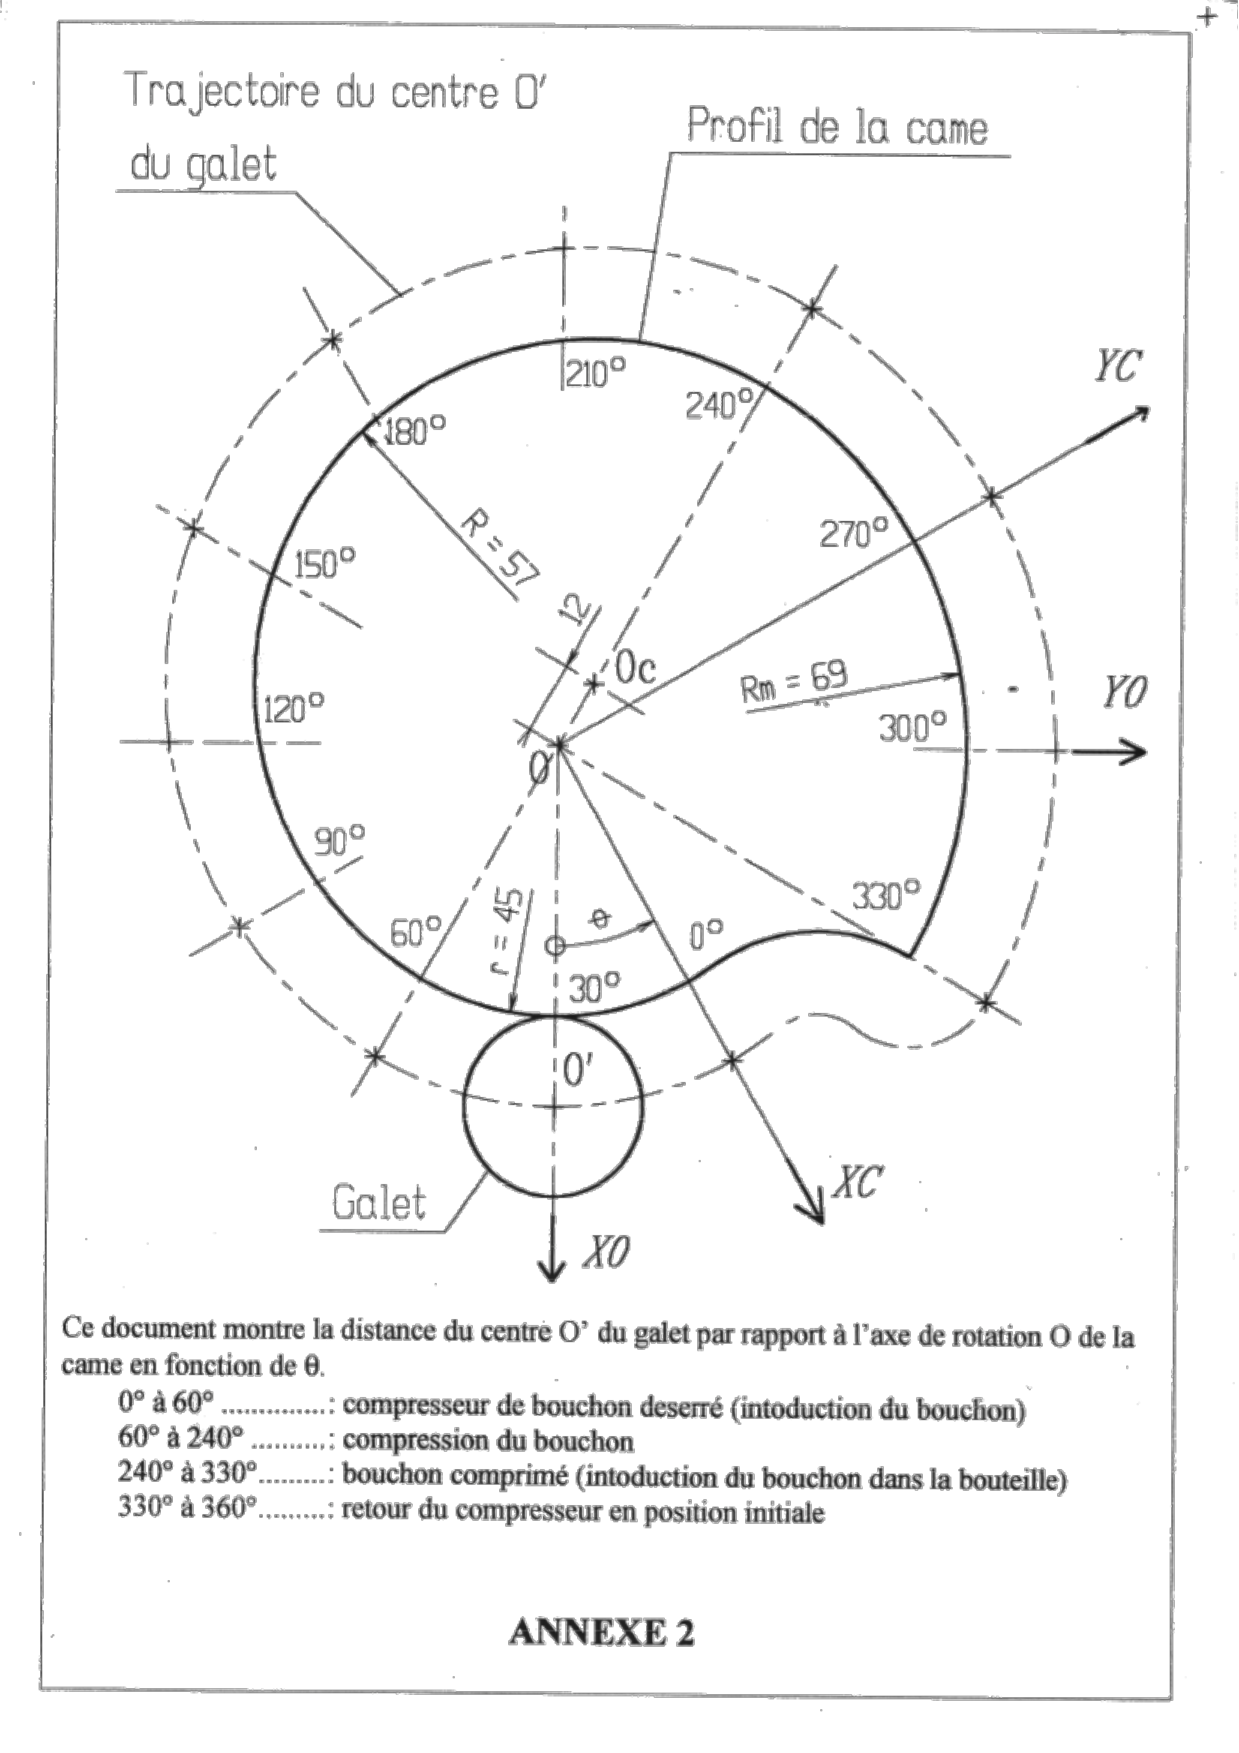
\includepdf[offset=-0.5cm -1cm]{img/Annexe2.pdf}

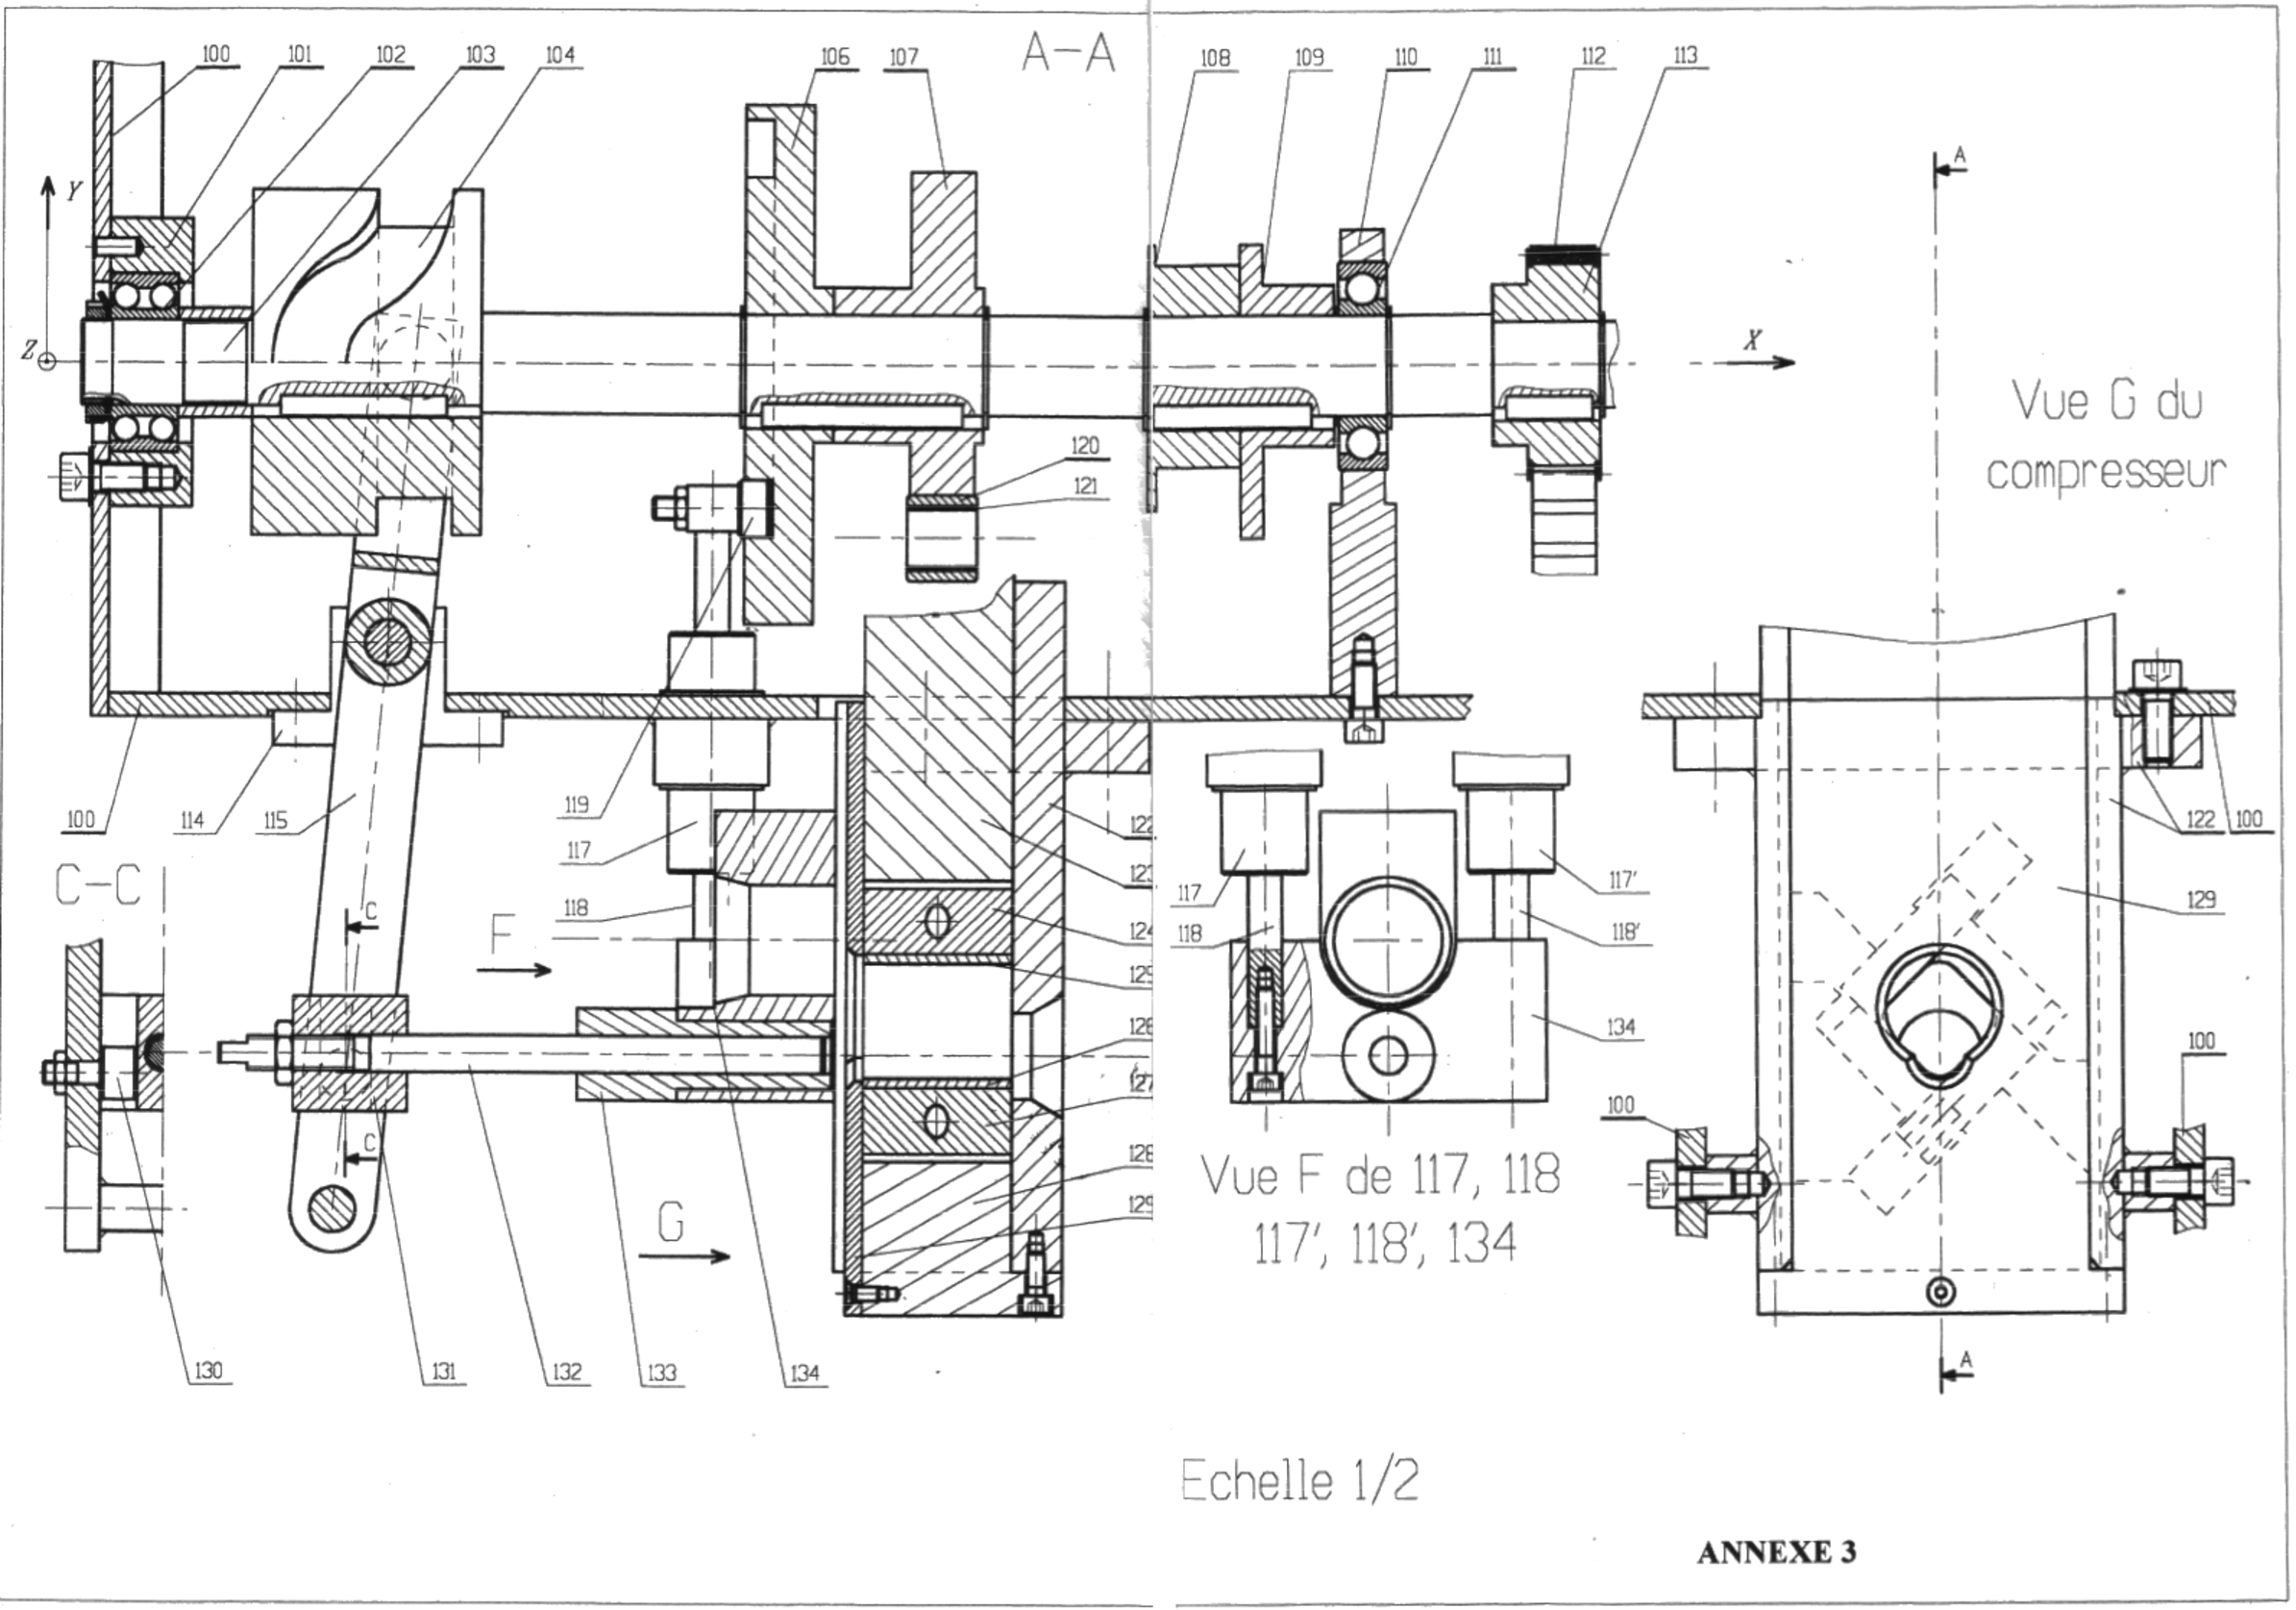
\includepdf[angle=90,offset=0.7cm -0.5cm]{img/Annexe3.pdf}

\cleardoublepage

\pagestyle{documentreponse}

\section{Documents réponse}

\reponse{3}{}{Le cas d'utilisation de ce système est de \og Boucher et Museler une bouteille \fg.}

\reponse{3}{}{On peut ajouter l'entreprise, un technicien/utilisateur.}

\reponse{3}{}{Sur le diagramme des Cas d'Utilisation, il n'y a que des acteurs.}

\reponse{3}{}{La pièce fait 2400tr/min, soit $\dot{\theta}=\frac{2400\cdot2\cdot\pi}{3600}=\frac{2\cdot2\cdot\pi}{3}\approx 4rad.s^{-1}$.}

%\newpage

\reponse{2}{\begin{center}
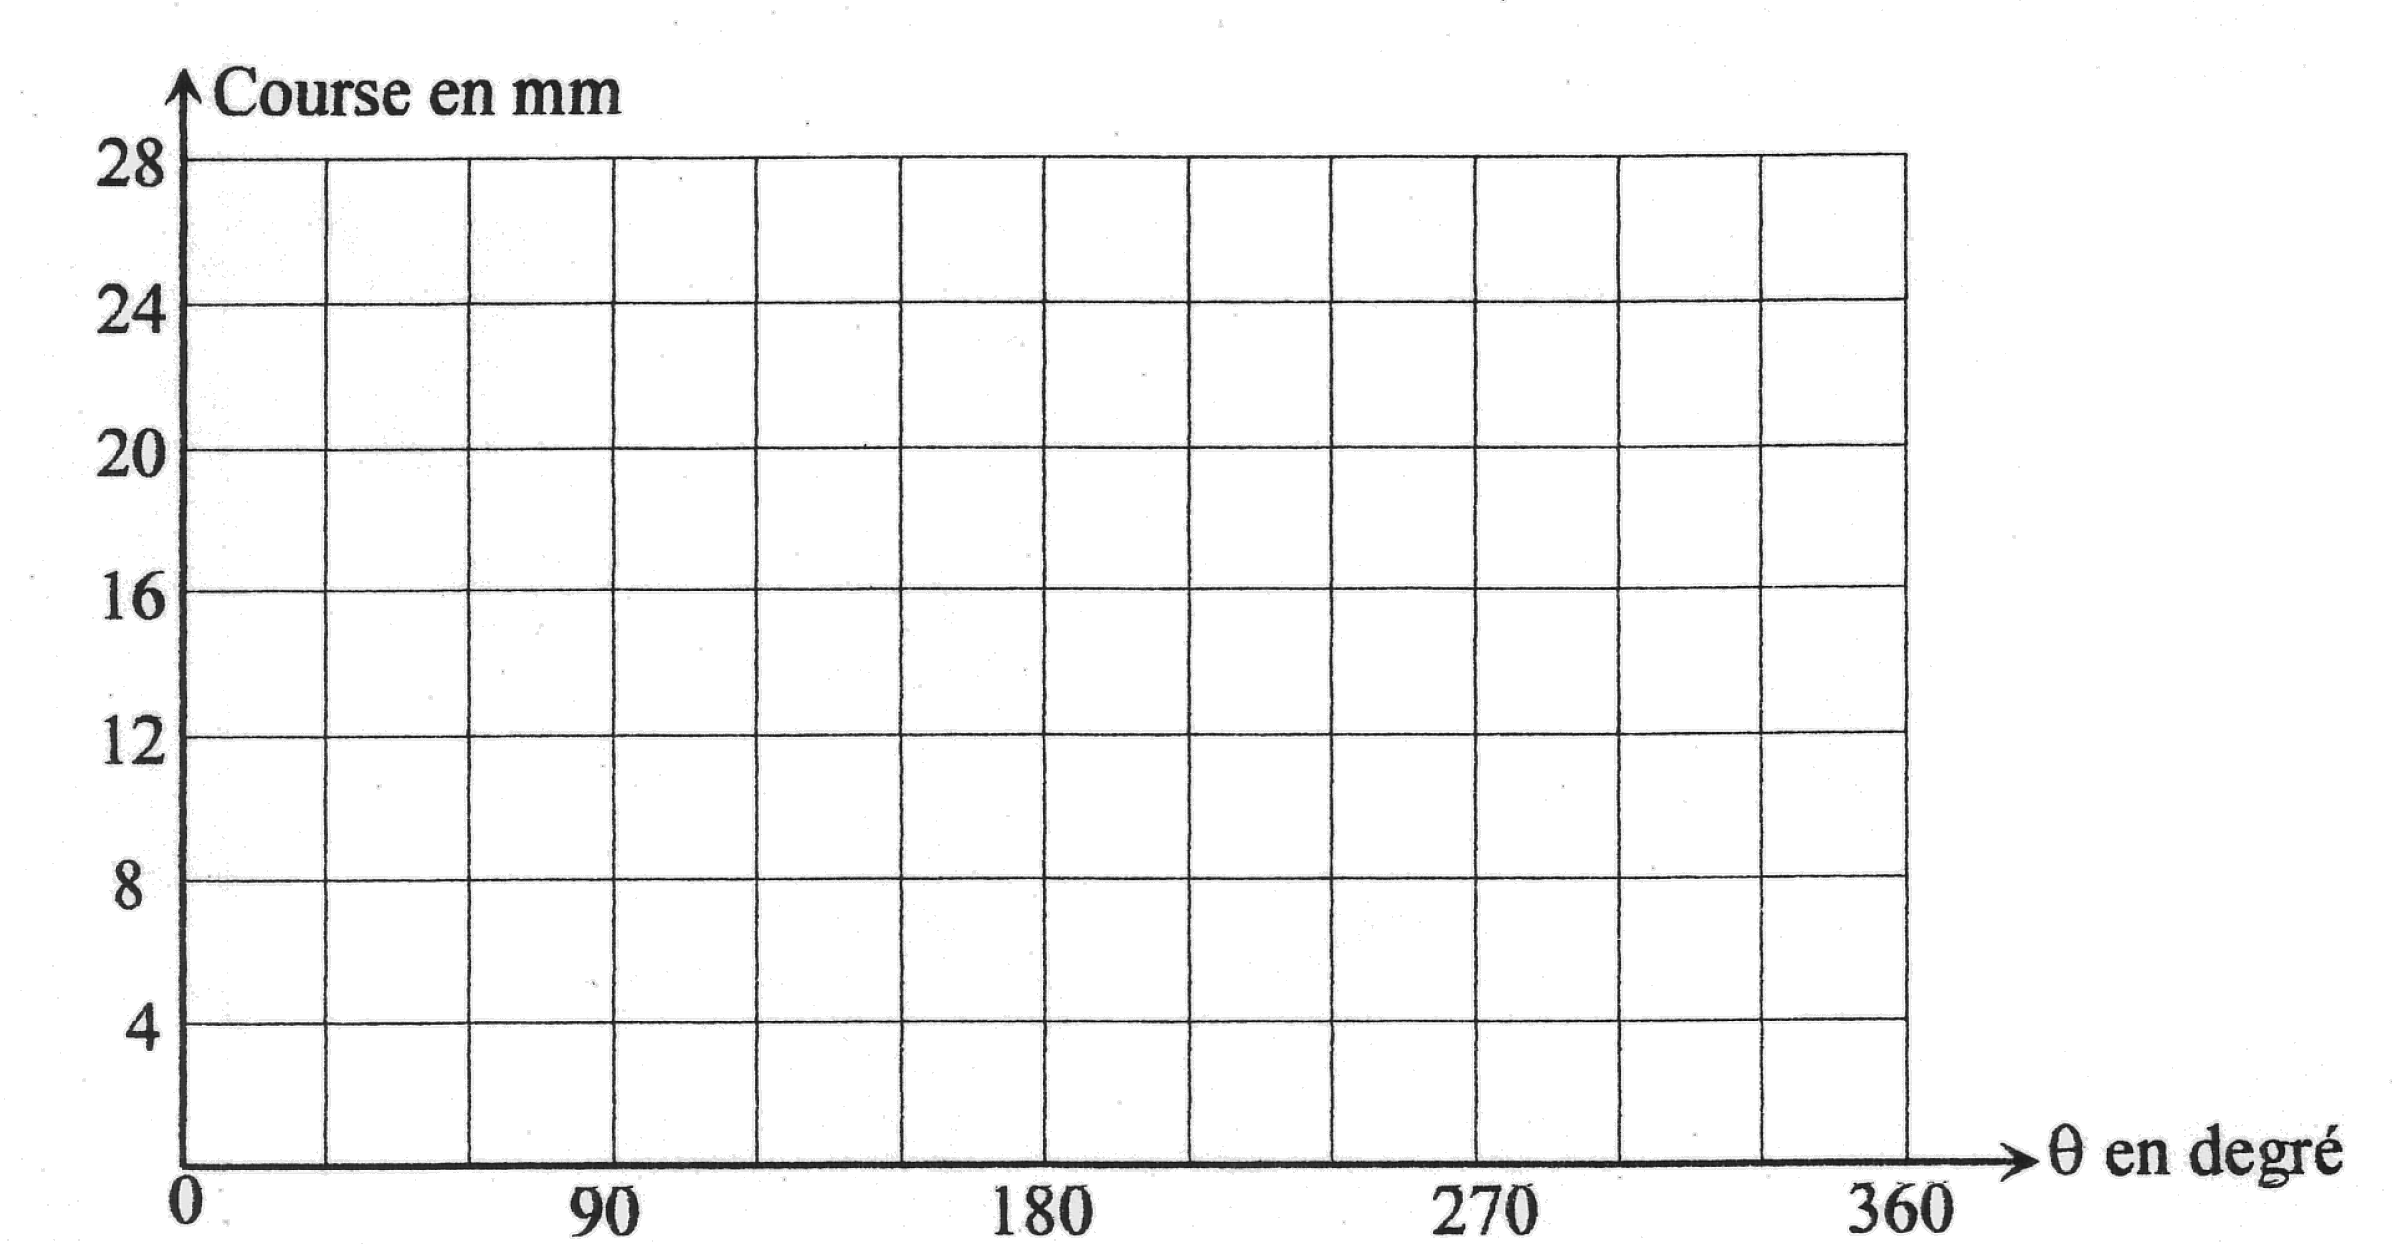
\includegraphics[width=0.7\linewidth]{img/dr01}
\end{center}}{

Course:
\begin{itemize}
 \item Entre 0° et 60 °: 0mm,
 \item Entre 60° et 240°: $\sqrt{12.cos(theta-60)-57)**2+(12.sin(theta2-60))**2}$,
 \item Entre 240° et 330°: 69mm.
\end{itemize}

\begin{center}
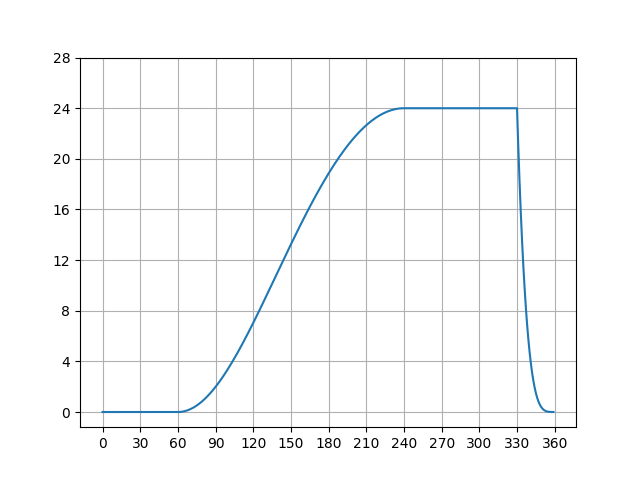
\includegraphics[width=0.7\linewidth]{img/dr01_cor}
\end{center}}

\reponse{0}{\begin{center}
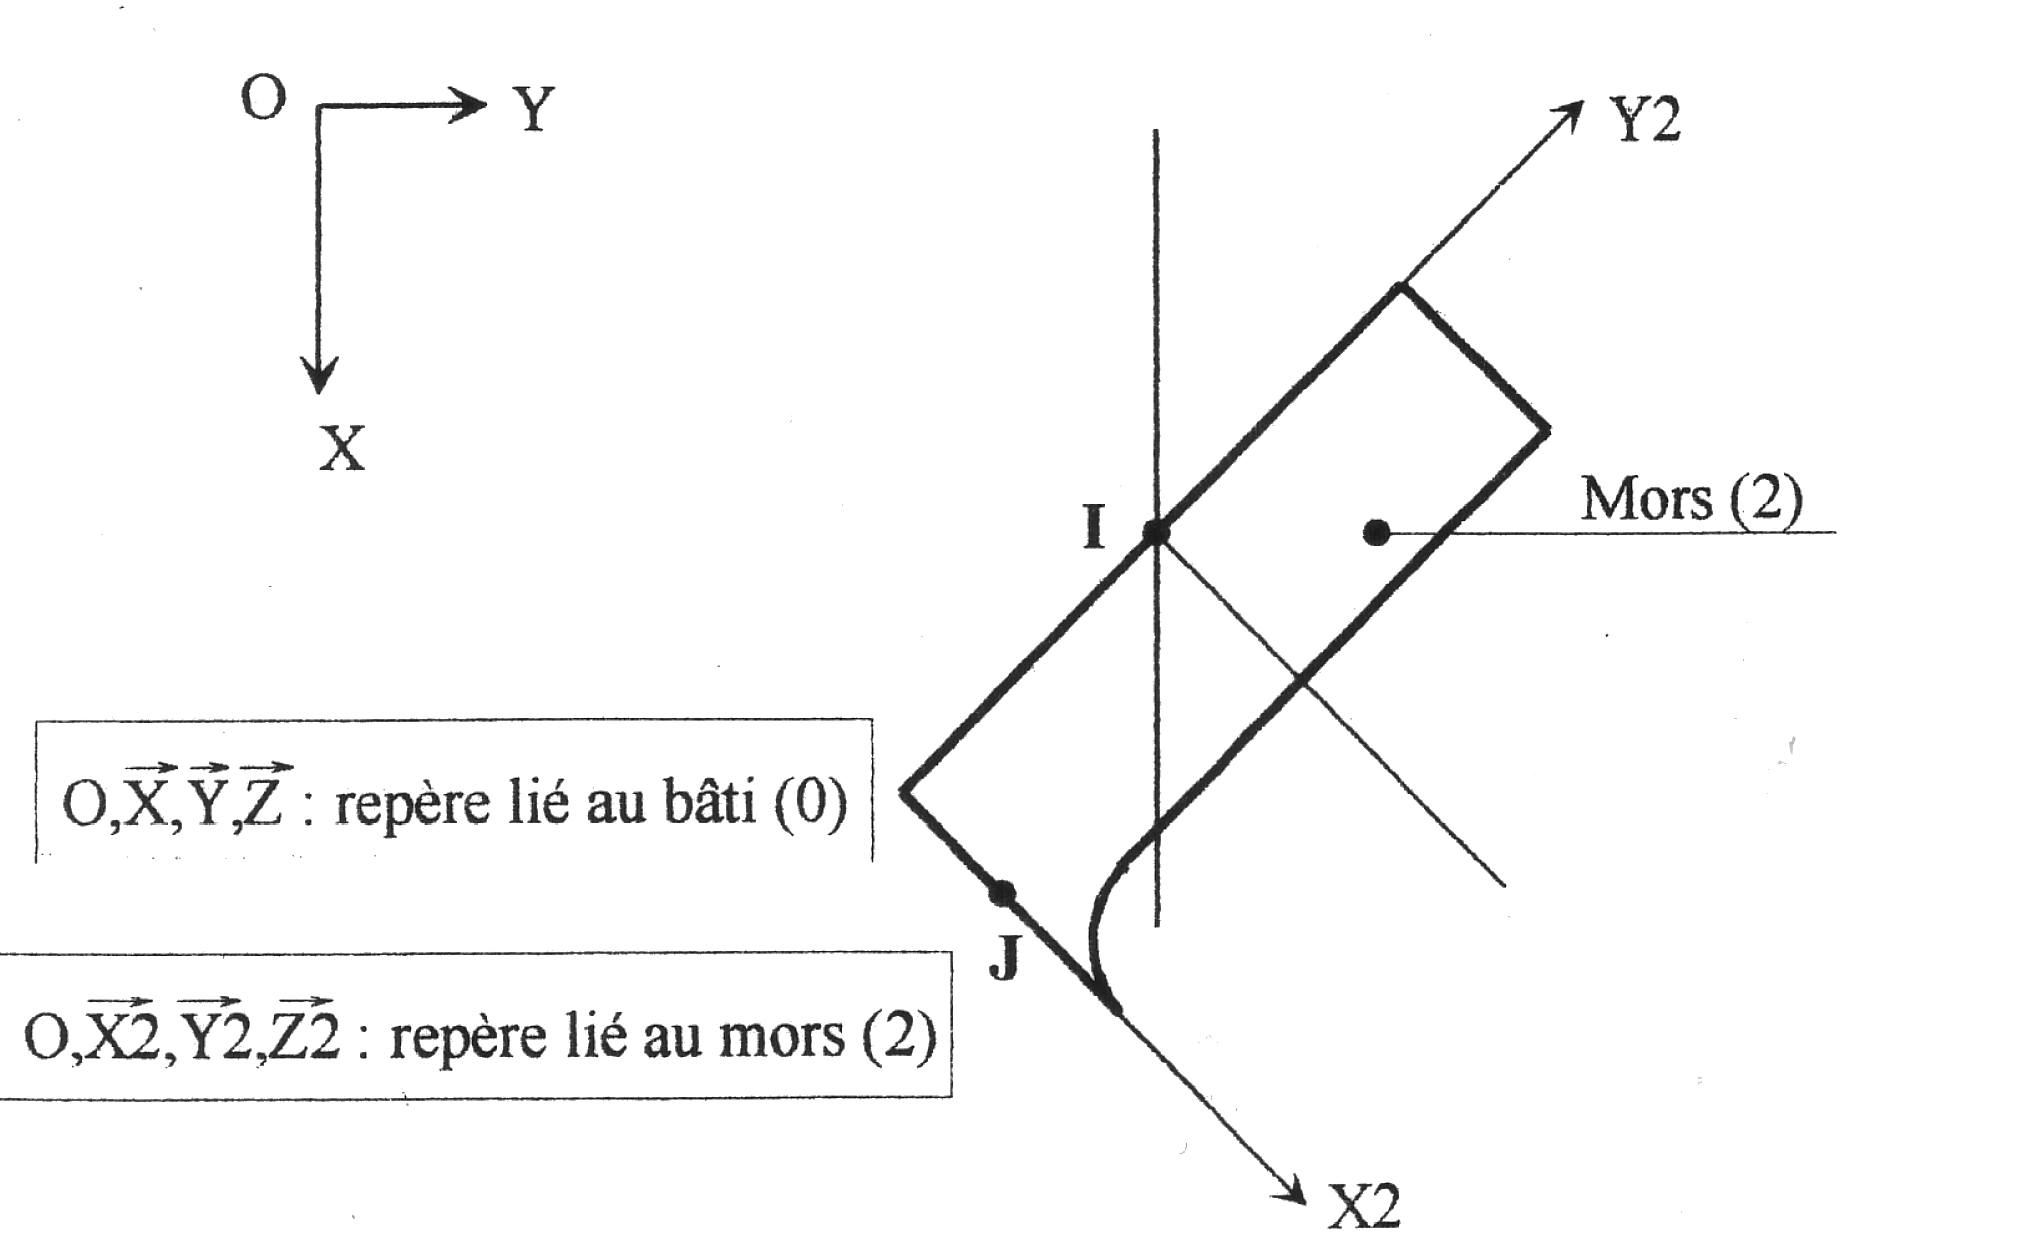
\includegraphics[width=0.8\linewidth]{img/dr02}
\end{center}}{\begin{center}
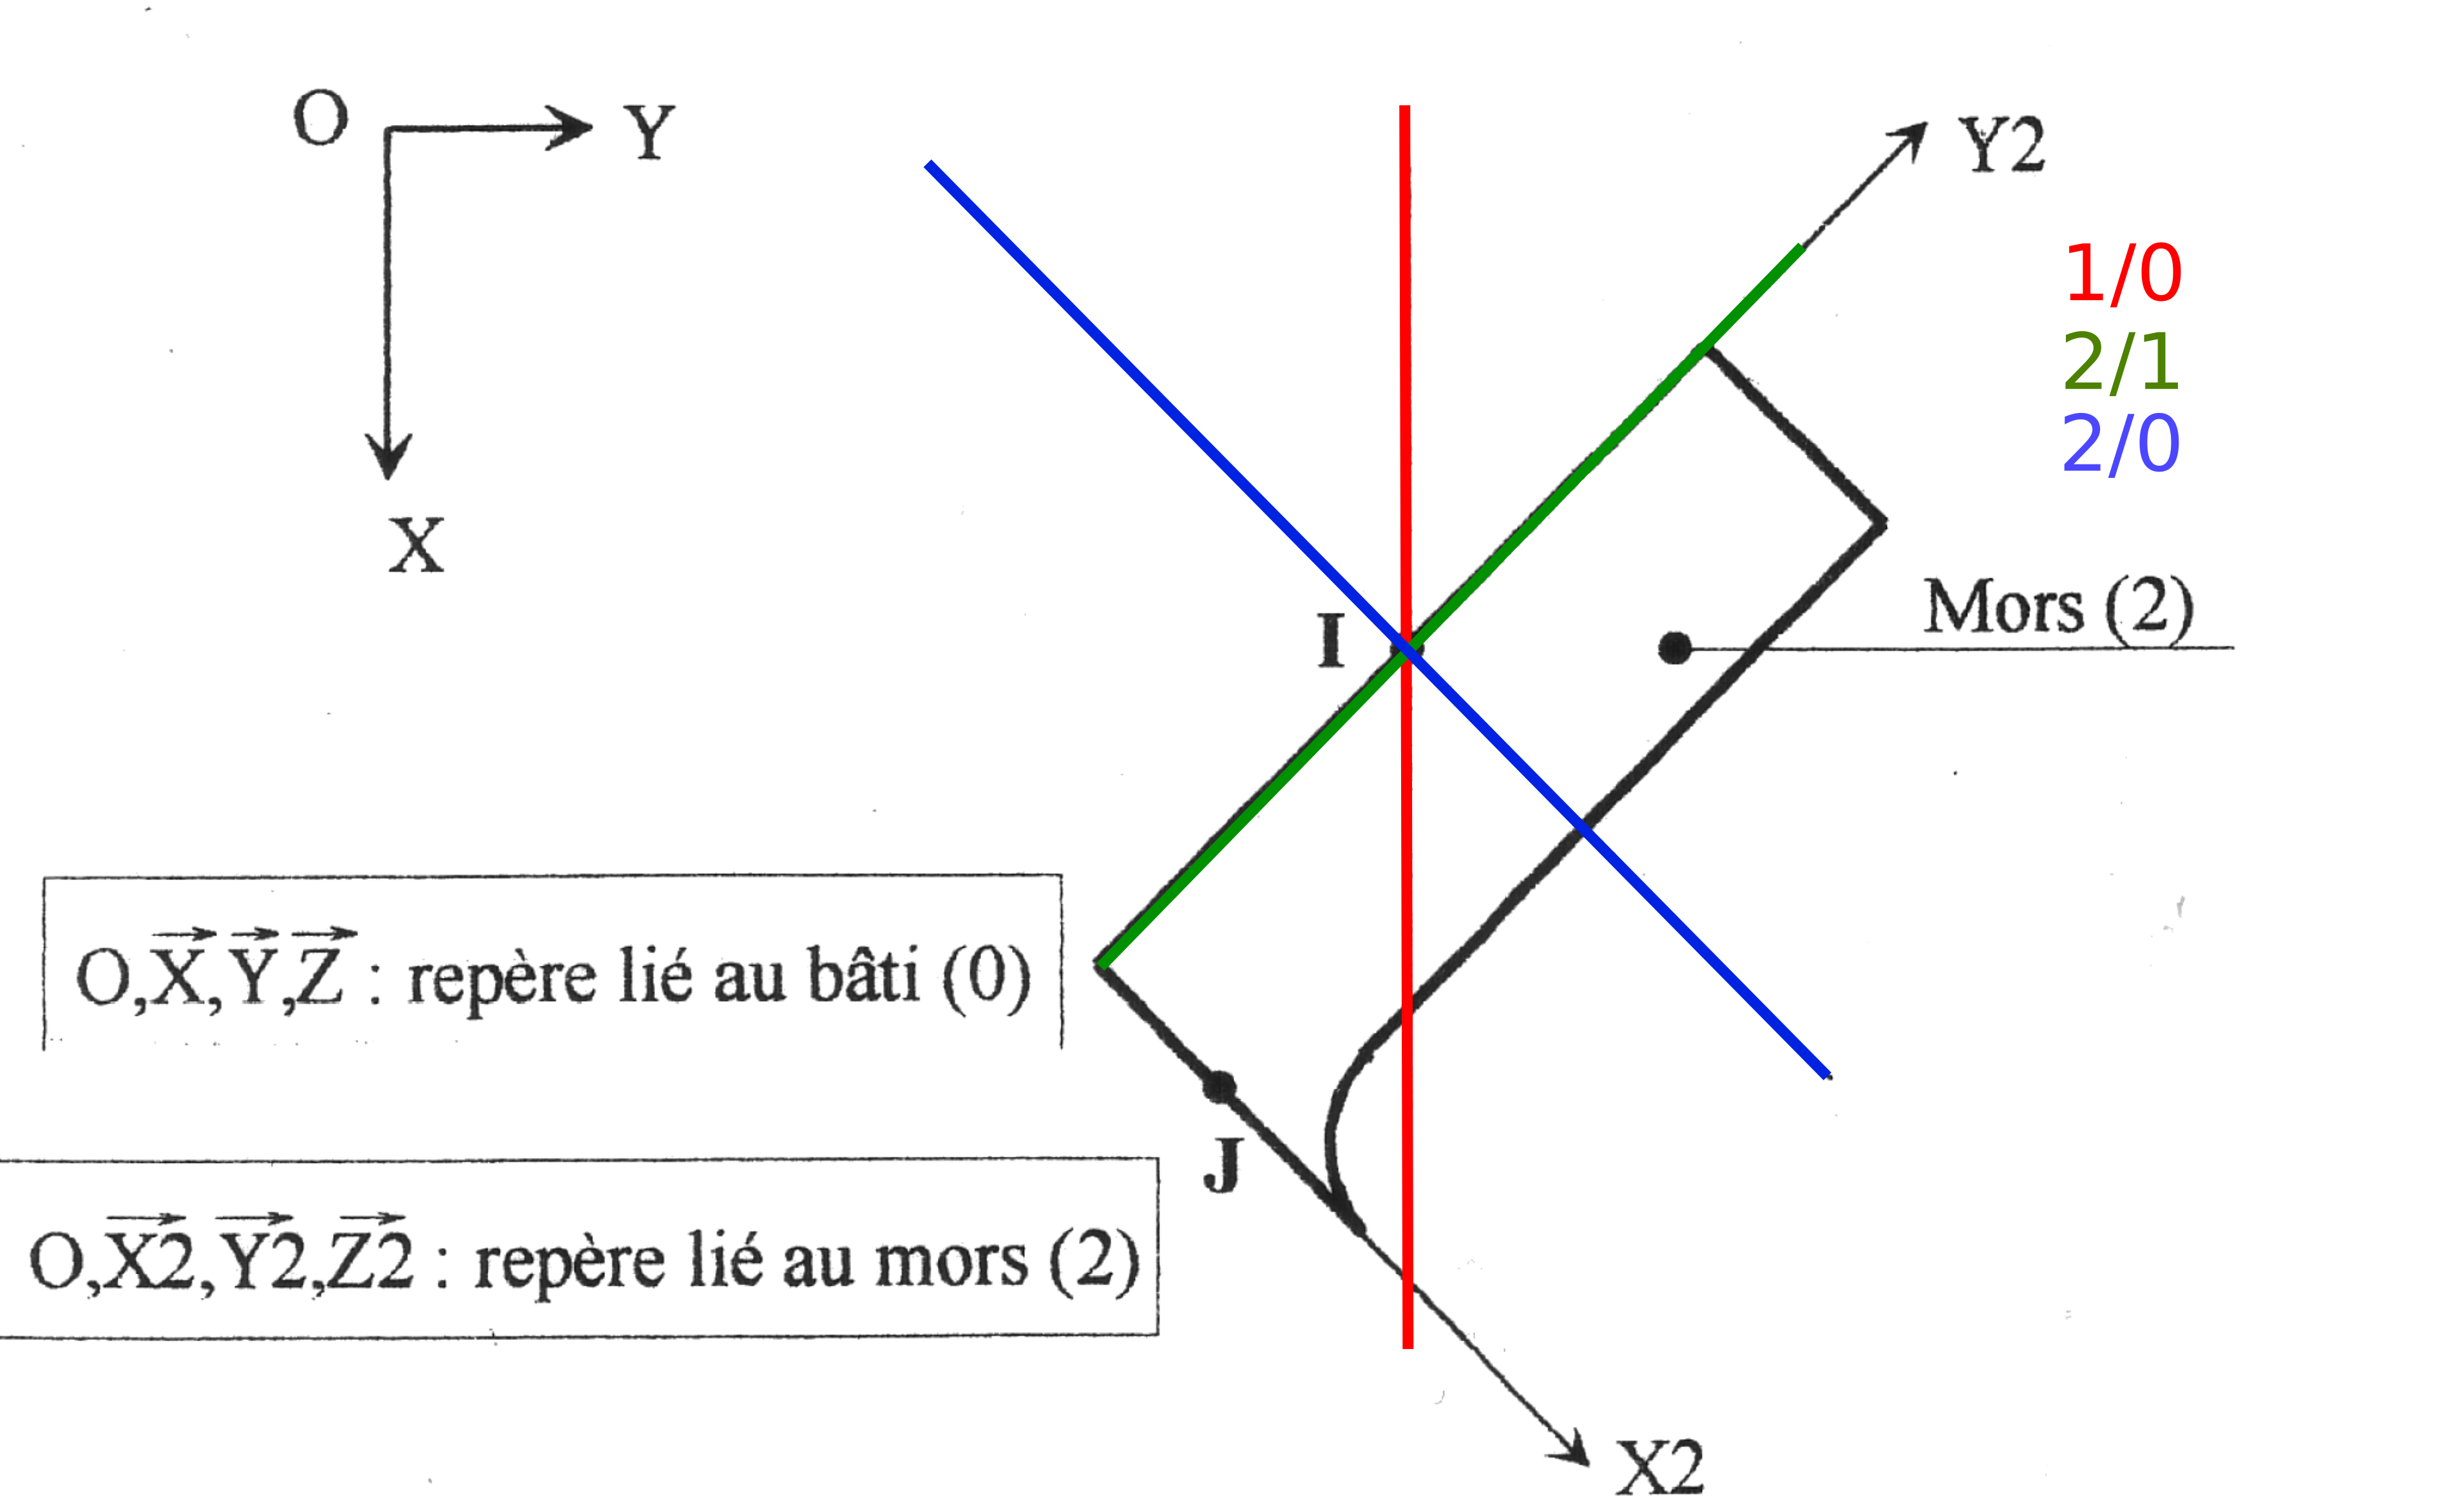
\includegraphics[width=0.8\linewidth]{img/dr02_cor}
\end{center}}

%\newpage

\reponse{4}{}{$\overrightarrow{V_{I\in 1/0}}.\overrightarrow{x}=V$

$\overrightarrow{V_{I\in 2/0}}=\overrightarrow{V_{I\in 2/1}}+\overrightarrow{V_{I\in 1/0}}$

$\overrightarrow{V_{I\in 2/0}}=V_{I\in 2/1}.\overrightarrow{Y_2}+V.\overrightarrow{X}$

$\overrightarrow{V_{I\in 2/0}}=V_{I\in 2/0}.\overrightarrow{X_2}$

or, $\overrightarrow{X}=\frac{\sqrt{2}}{2}.\overrightarrow{X_2}-\frac{\sqrt{2}}{2}.\overrightarrow{Y_2}$


Donc, $\overrightarrow{V_{I\in 2/0}}=V.\frac{\sqrt{2}}{2}.\overrightarrow{X_2}$ et $\overrightarrow{V_{I\in 2/1}}=V.\frac{\sqrt{2}}{2}.\overrightarrow{Y_2}$.
}

\reponse{11}{}{
\begin{enumerate}
 \item $\overrightarrow{X_i}=cos\alpha.\overrightarrow{X}+sin\alpha.\overrightarrow{Y}$
 \item $\overrightarrow{OO'}.\overrightarrow{Y}=(\overrightarrow{OO_C}+\overrightarrow{O_CI}+\overrightarrow{IO'}).\overrightarrow{Y}=0$,
 
 $(-e.\overrightarrow{X_C}+R.\overrightarrow{X_i}+r.\overrightarrow{X_i}).\overrightarrow{Y}=0$
 
$-e.sin\theta+(R+r).cos\theta=0$, donc $\alpha=arcsin(\frac{e.sin\theta}{R+r})$
 \item $\overrightarrow{V_{I\in C/0}}=\overrightarrow{V_{O\in C/0}}+\overrightarrow{IO}\wedge\overrightarrow{\Omega_{C/0}}$
 
 $\overrightarrow{V_{I\in C/0}}=(-R.\overrightarrow{X_i}+e.\overrightarrow{X_c})\wedge\dot{\theta}\overrightarrow{z}$
 
  $\overrightarrow{V_{I\in C/0}}=\left[(-R.sin\alpha+e.sin\theta).\overrightarrow{X}+(R.cos\alpha-e.cos\theta).\overrightarrow{Y}\right].\dot{\theta}$
 
 $\overrightarrow{V_{I\in C/0}}=\overrightarrow{V_{I\in C/G}}+\overrightarrow{V_{I\in G/0}}=\overrightarrow{V_{I\in G/0}}$

 $\overrightarrow{V_{O’\in G/0}}=\overrightarrow{V_{I\in G/0}}+\overrightarrow{O’I}\wedge \overrightarrow{\Omega_{G/0}}$
 
 $\overrightarrow{O'I}\wedge\overrightarrow{\Omega_{G/0}}=-r.\overrightarrow{X_i}\wedge\omega_G.\overrightarrow{z}$

 $\overrightarrow{O'I}\wedge\overrightarrow{\Omega_{G/0}}=-r.(cos\alpha\overrightarrow{X}+sin\alpha\overrightarrow{Y})\wedge\omega_G.\overrightarrow{z}$

 $\overrightarrow{O'I}\wedge\overrightarrow{\Omega_{G/0}}=-r.\omega_G.(-cos\alpha\overrightarrow{Y}+sin\alpha\overrightarrow{X})$

 $\overrightarrow{V_{O'\in G/0}}.\overrightarrow{Y}=0$, donc  
$\overrightarrow{V_{O'\in G/0}}=V_X.\overrightarrow{X}$ et 
 
$(R.cos\alpha-e.cos\theta).\dot{\theta}+r.cos\alpha.\omega_G=0$, donc

$\omega_G=\frac{(e.cos\theta-R.cos\alpha).\dot{\theta}}{r.cos\alpha.}$

$V_X=(-R.sin\alpha+e.sin\theta).\dot{\theta}-r.sin\alpha.\omega_G$


$\left\{V_{G/0}\right\}=\left\{\begin{array}{cc}
 0 & V_X \\ 0 & 0 \\ \omega_G & 0 \end{array}\right\}_{O',\left(\overrightarrow{X},\overrightarrow{Y},\overrightarrow{Z}\right)}$
\end{enumerate}

}

\reponse{2}{}{
$\|\overrightarrow{E_{R\rightarrow 2}}\|=k.\Delta l=k.(L-L_0)$

En fin de compression, $\|\overrightarrow{E_{R\rightarrow 2}}\|=4.(50-30)=80N$
}

%\newpage

\reponse{2}{\begin{center}
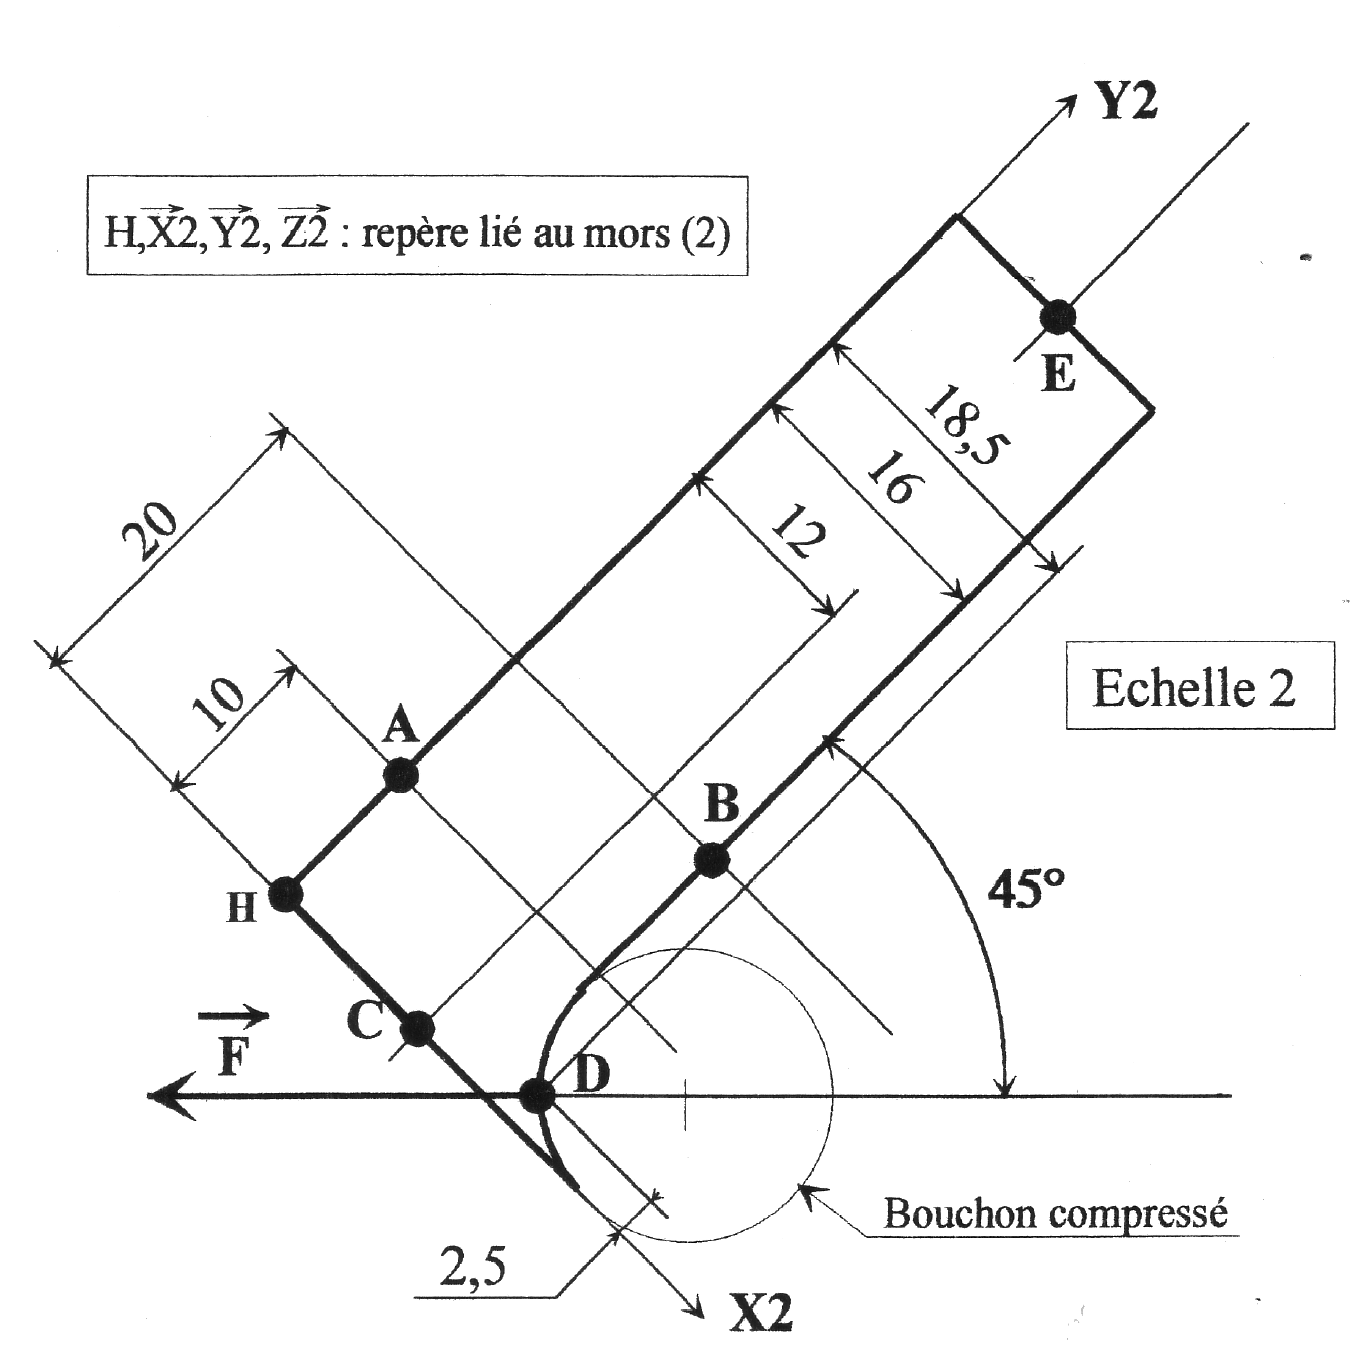
\includegraphics[width=0.5\linewidth]{img/dr03}
\end{center}}{\begin{center}
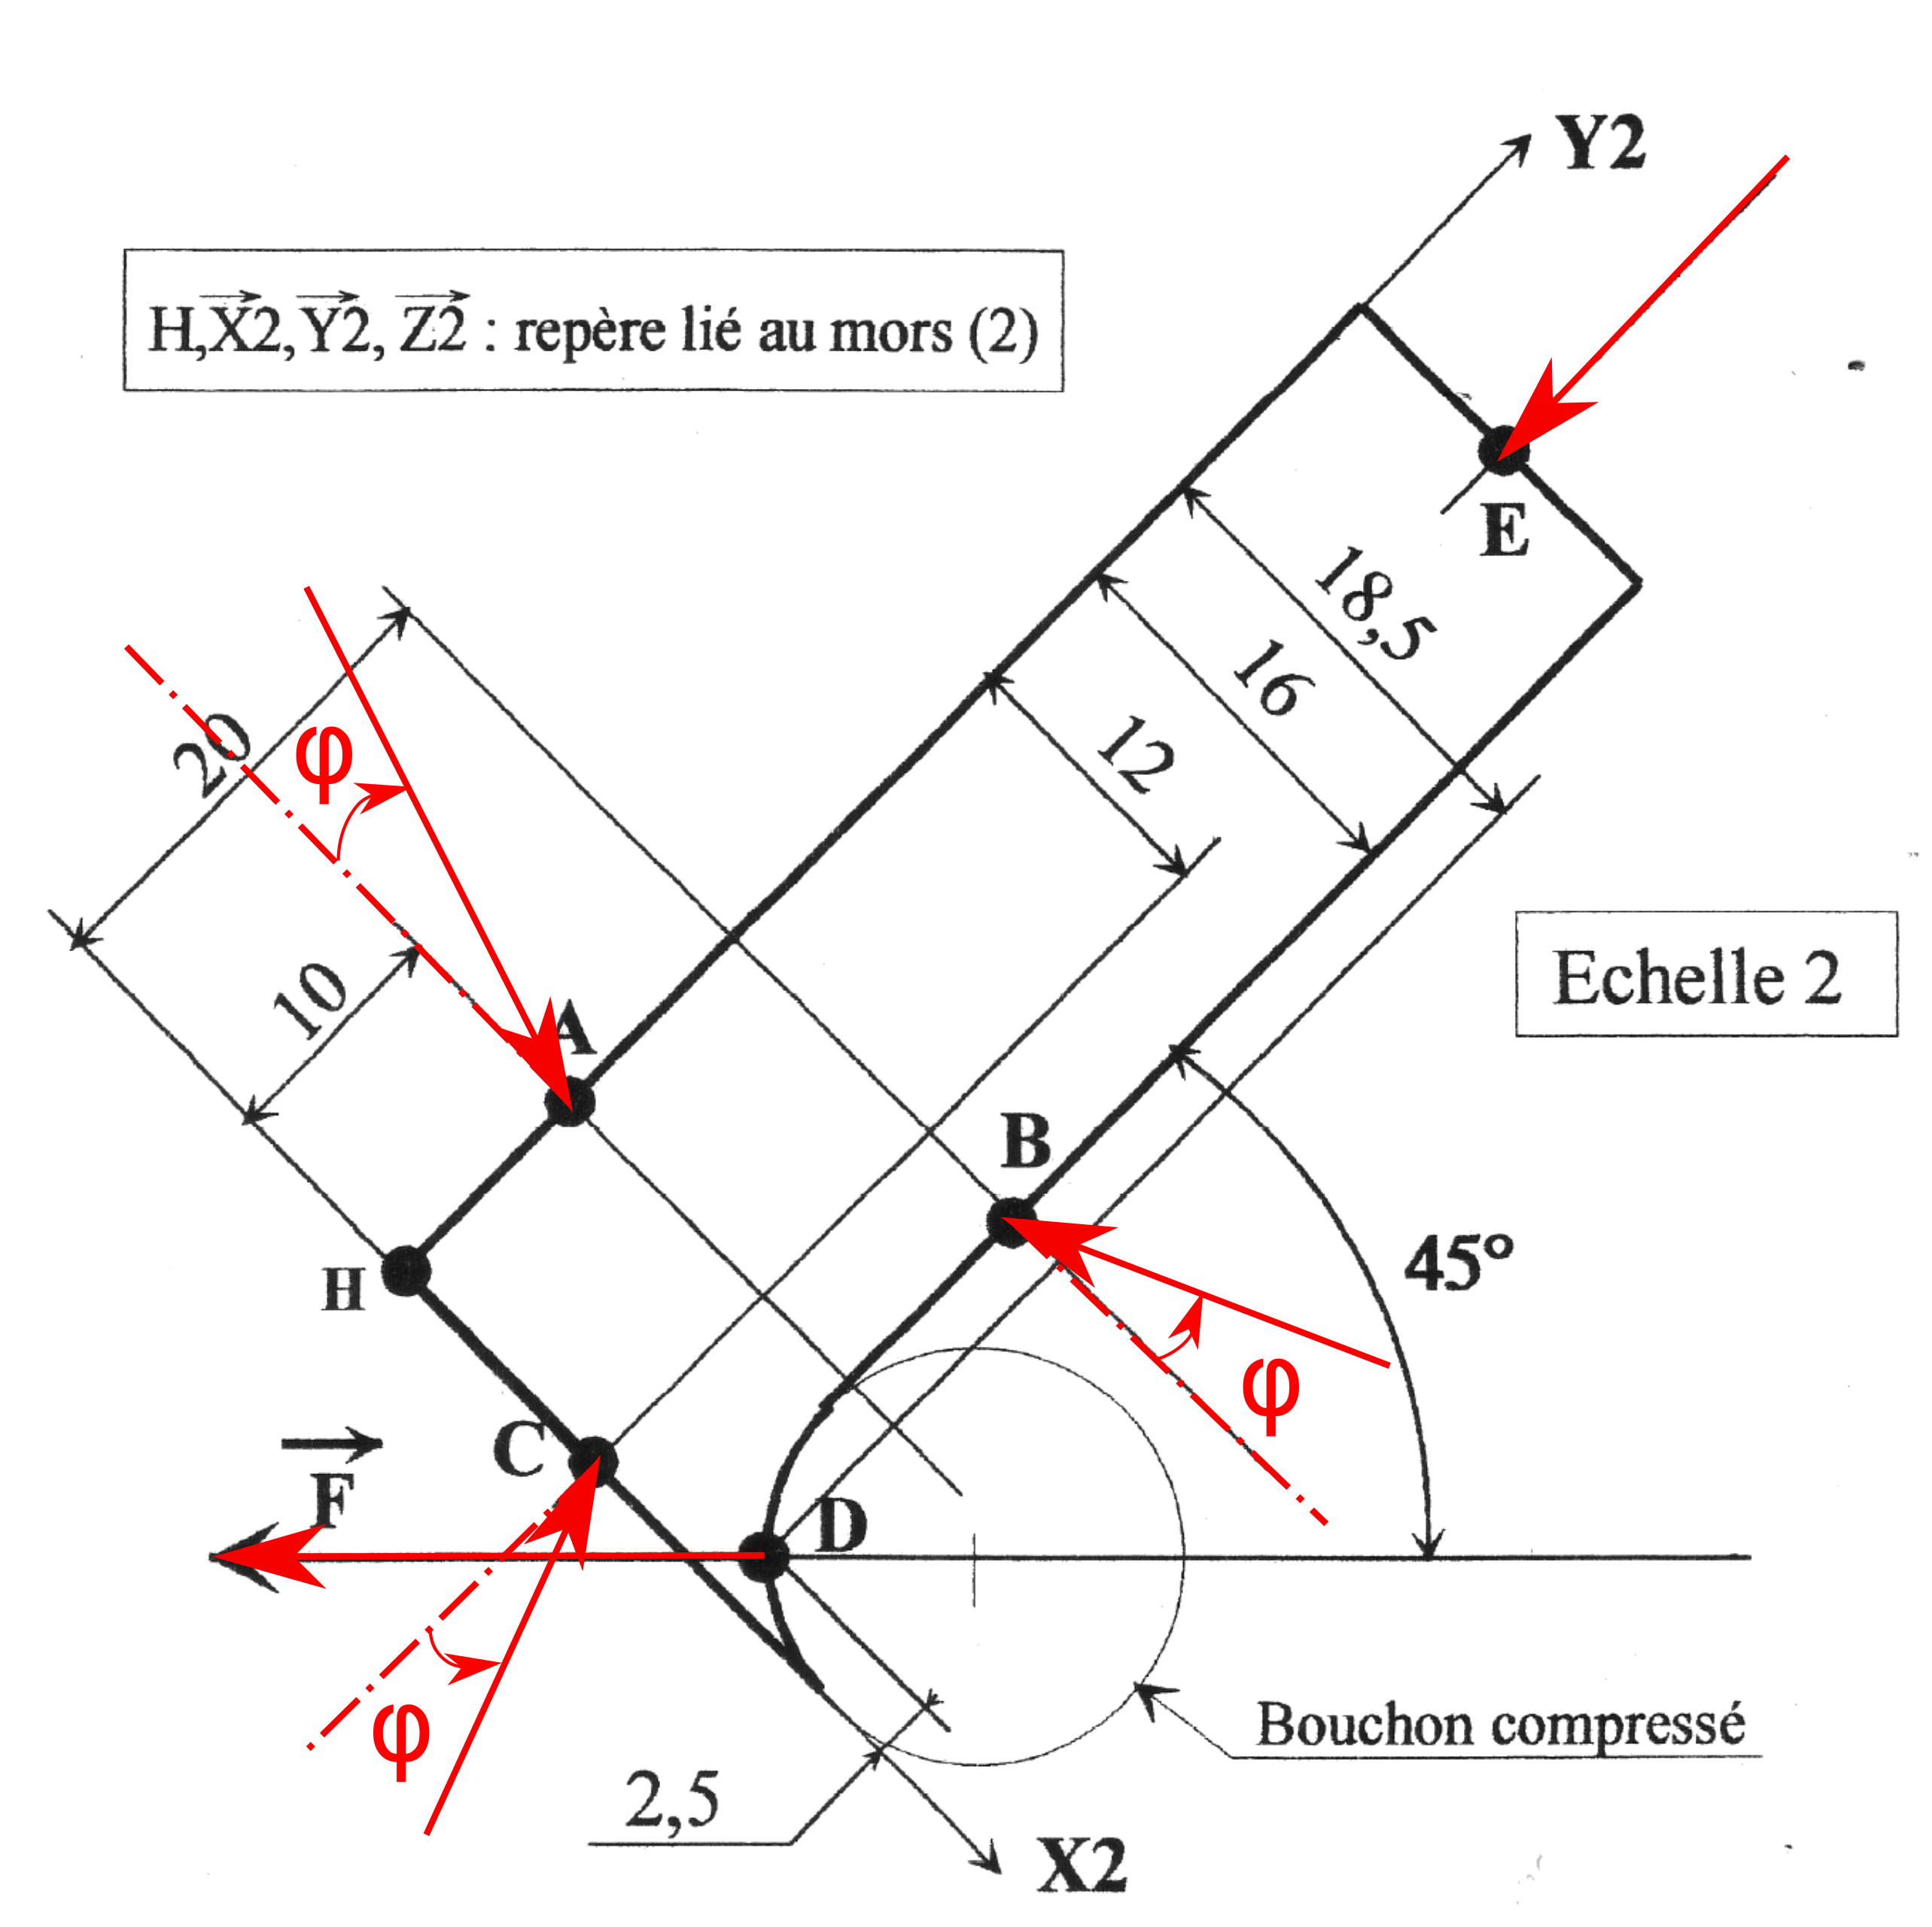
\includegraphics[width=0.5\linewidth]{img/dr03_cor}
\end{center}}

\reponse{8}{}{
Résultante:\\
$A_{12}.cos\varphi.\overrightarrow{X_2}-A_{12}.sin\varphi.\overrightarrow{Y_2}
-B_{32}.cos\varphi.\overrightarrow{X_2}-B_{32}.sin\varphi.\overrightarrow{Y_2}
+C_{52}.cos\varphi.\overrightarrow{Y_2}-C_{52}.sin\varphi.\overrightarrow{X_2}
-F.\frac{\sqrt{2}}{2}.\overrightarrow{X_2}-F.\frac{\sqrt{2}}{2}.\overrightarrow{Y_2}
+E_R.\overrightarrow{Y_2}=\overrightarrow{0}$

$A_{12}.cos\varphi-B_{32}.cos\varphi-C_{52}.sin\varphi-F.\frac{\sqrt{2}}{2}=0$

$-A_{12}.sin\varphi-B_{32}.sin\varphi+C_{52}.cos\varphi-F.\frac{\sqrt{2}}{2}+E_R=0$

Moment:\\
$-10\cdot A_{12}\cdot cos\varphi+20\cdot B_{32}\cdot cos\varphi-16\cdot B_{32}\cdot sin\varphi 
+12\cdot C_{52}\cdot cos\varphi -18,5\cdot F\cdot \frac{\sqrt{2}}{2} +2,5\cdot F\cdot \frac{\sqrt{2}}{2}-8.E=0$}

%\newpage

\reponse{20}{}{Isoler 1:\\ B.A.M: $0\rightarrow 1 (négligée), 2\rightarrow 1, 3\rightarrow 1, G\rightarrow 1$

$\overrightarrow{F_{3\rightarrow 1}}.\overrightarrow{x}+\overrightarrow{A_{\rightarrow 1}}.\overrightarrow{x}+\overrightarrow{R_{G\rightarrow 1}}.\overrightarrow{x}=0$

$-10000-13585.\frac{\sqrt{2}}{2}-679.\frac{\sqrt{2}}{2}+\overrightarrow{R_{G\rightarrow 1}}.\overrightarrow{X}=0$

$R_{G\rightarrow 1}=20086,2$

Isoler G:\\ B.A.M: $1\rightarrow G, C\rightarrow G$

$\overrightarrow{R_{1\rightarrow G}}+\overrightarrow{R_{C\rightarrow G}}=\overrightarrow{0}$

Donc $\|\overrightarrow{R_{C\rightarrow G}}\|=20086,2N$


}

\reponse{2}{}{$E(p)=U(p)-R.I(p)=Ke.\Omega(p)$\\$Cm(p)=Kt.I(p)=J.p.\Omega(p)$}

\reponse{0}{\begin{center}
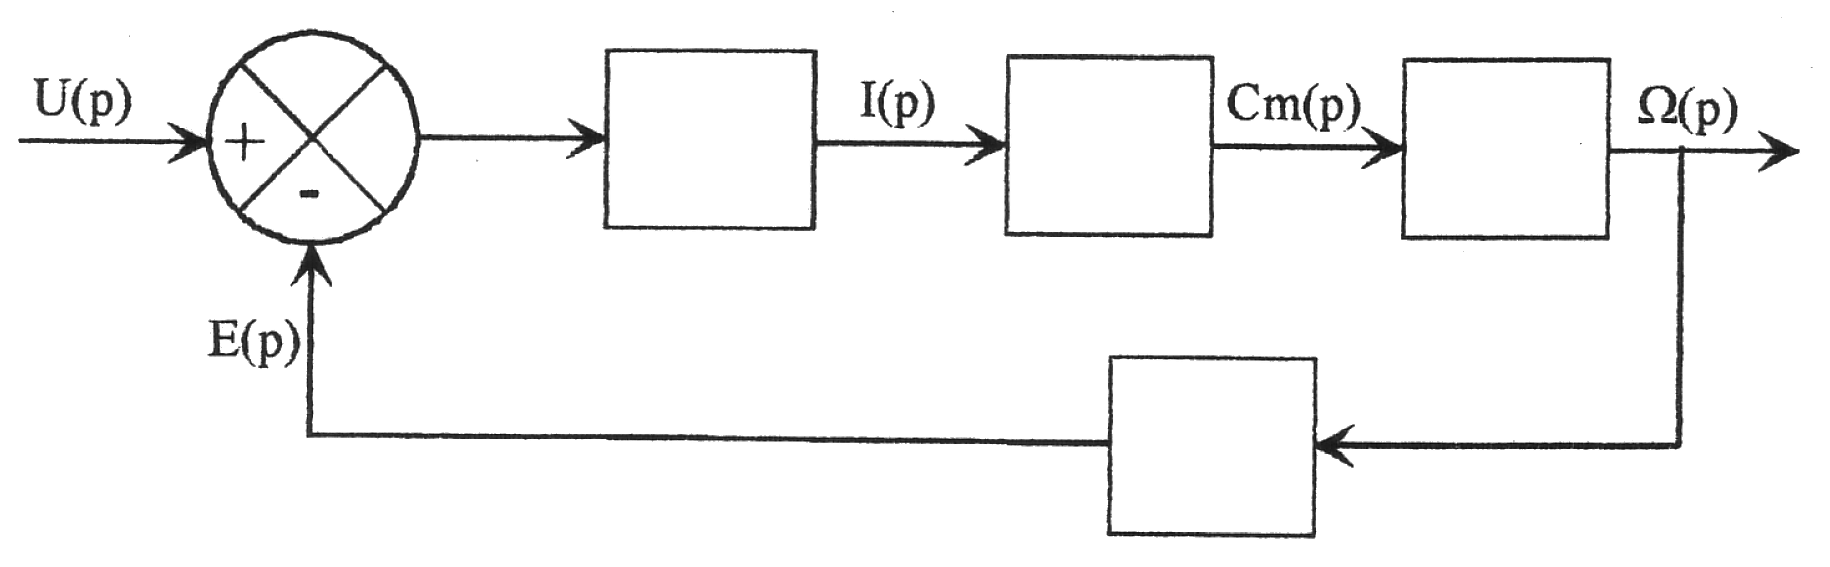
\includegraphics[width=0.7\linewidth]{img/dr04}
\end{center}}{\begin{center}
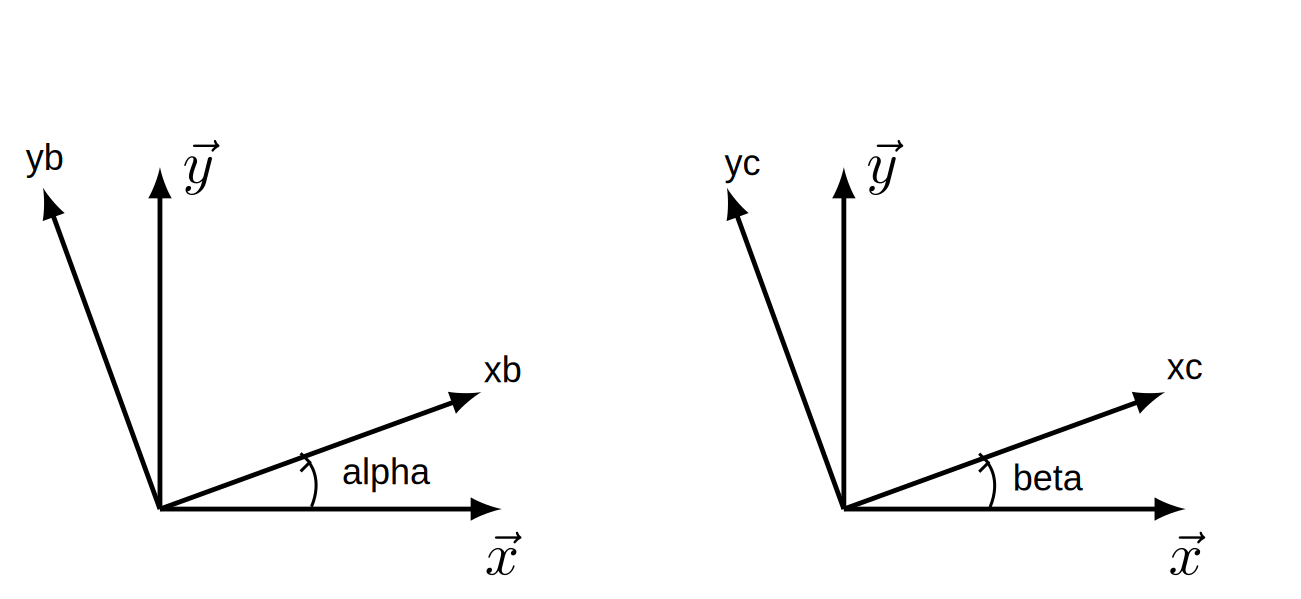
\includegraphics[width=0.7\linewidth]{img/dr04_cor}
\end{center}}

\reponse{3}{}{$\frac{\Omega(p)}{U(p)}=\frac{\frac{1}{Ke}}{1+\frac{R.J}{Ke.Kt}.p}$}

\reponse{3}{}{Il s'agit d'un ordre 1 car le déphasage va de 0° à -90°, et que la pente sur la courbe du gain est de -20dB/dec.

$20.log(Ks)=-6$, donc $Ks=10^{\frac{-3}{10}}\approx0,5$ et $\tau=\frac{1}{20}=0,05s$}

\reponse{3}{}{
$Ke=\frac{1}{0,5}=2V.rad^{-1}.s$ et $\frac{R.J}{Ke.Kt}=0,05$, donc $J=\frac{2\cdot0,05\cdot0,85}{3,4}=0,025kg.m^2$.
}


%\newpage

\reponse{3}{}{
$t_{R,5\%}=3.\tau=0,15s$

$K=\frac{110}{0,05}=2200rad.s^2$
}

\reponse{3}{\begin{center}
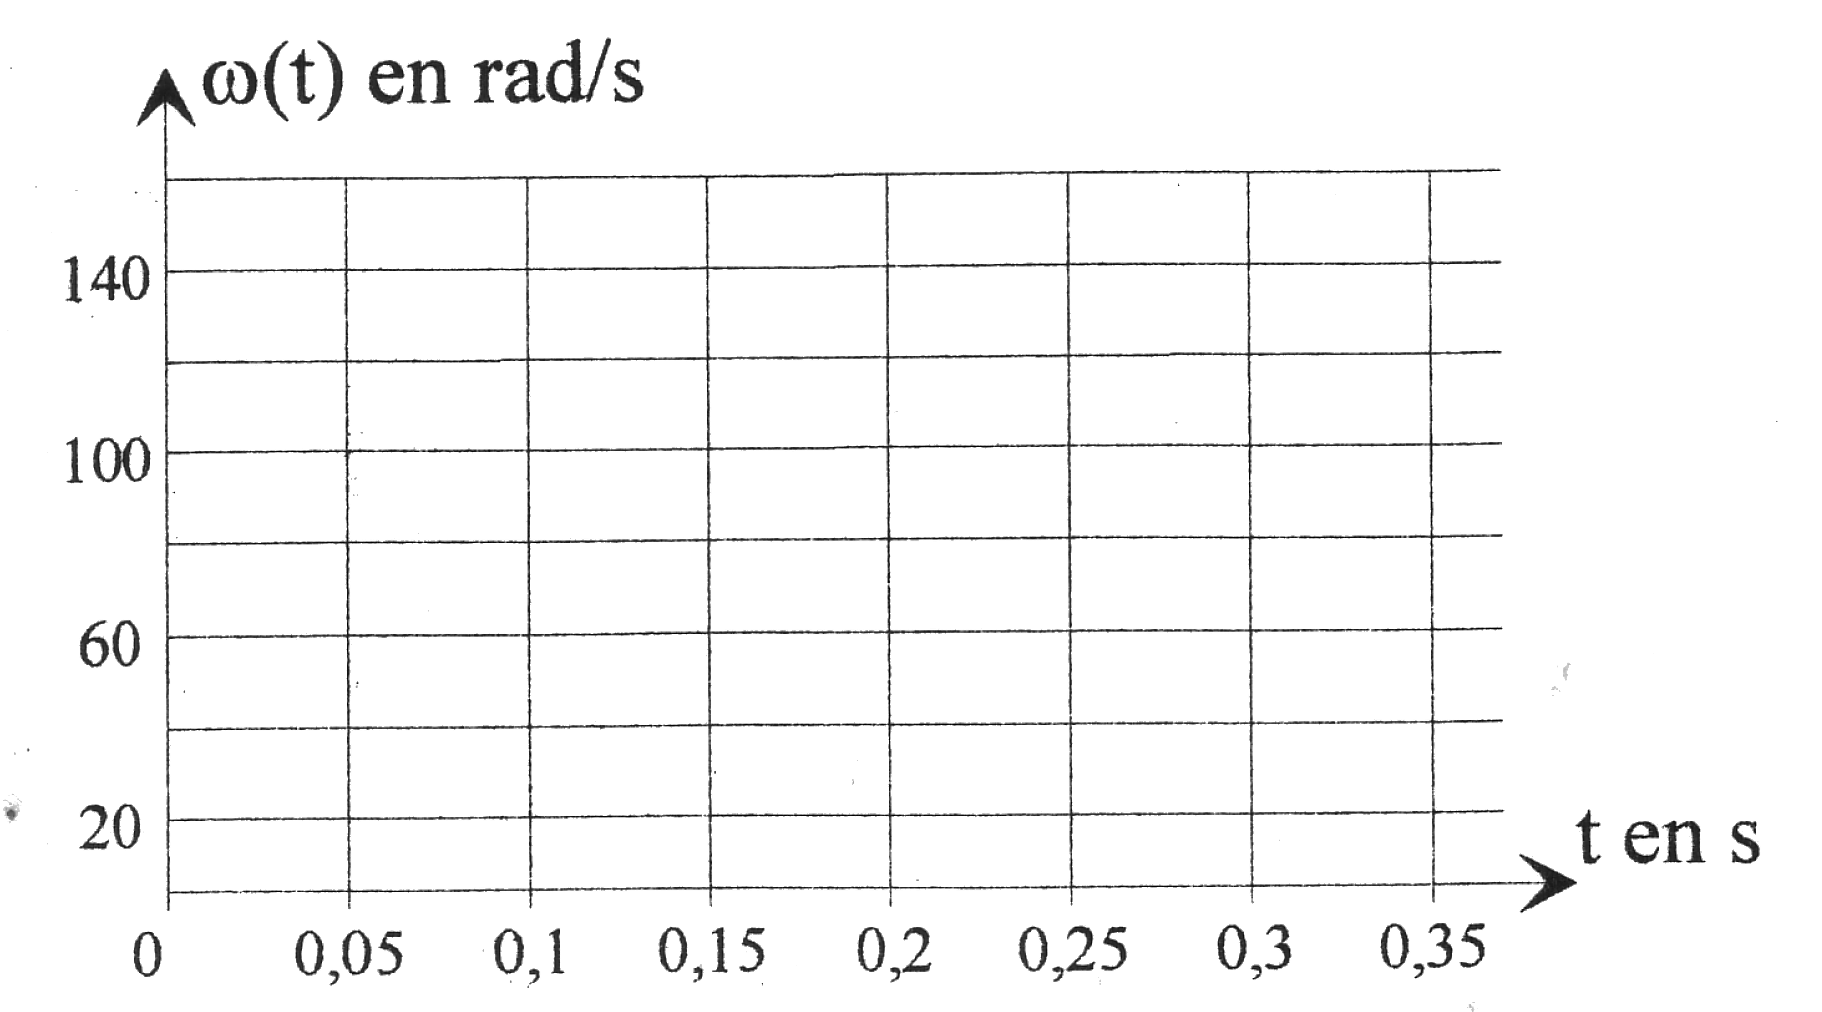
\includegraphics[width=0.7\linewidth]{img/dr05}
\end{center}}{\begin{center}
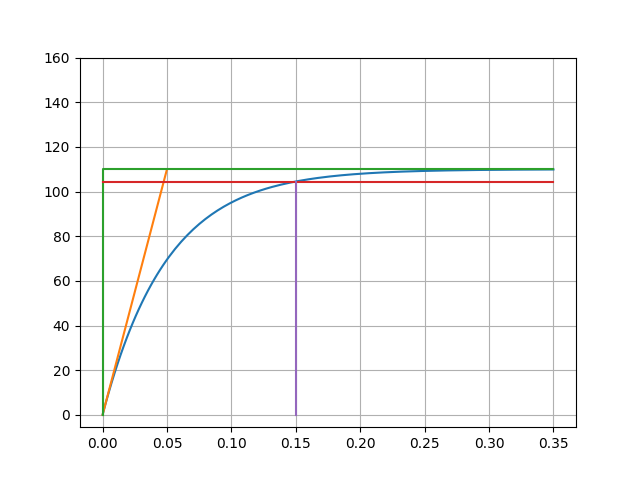
\includegraphics[width=0.7\linewidth]{img/dr05_cor}
\end{center}}

\reponse{3}{}{$F(p)=Kc\cdot\frac{Ka\cdot H(p)}{1+Ka\cdot Kc\cdot H(p)}=0,06\cdot\frac{0,5\cdot Ka}{1+0,05\cdot p+Ka\cdot0,06\cdot0,5}=\frac{0,03\cdot Ka}{(1+0,03\cdot Ka)+0,05\cdot p}$}

\reponse{3}{\begin{center}
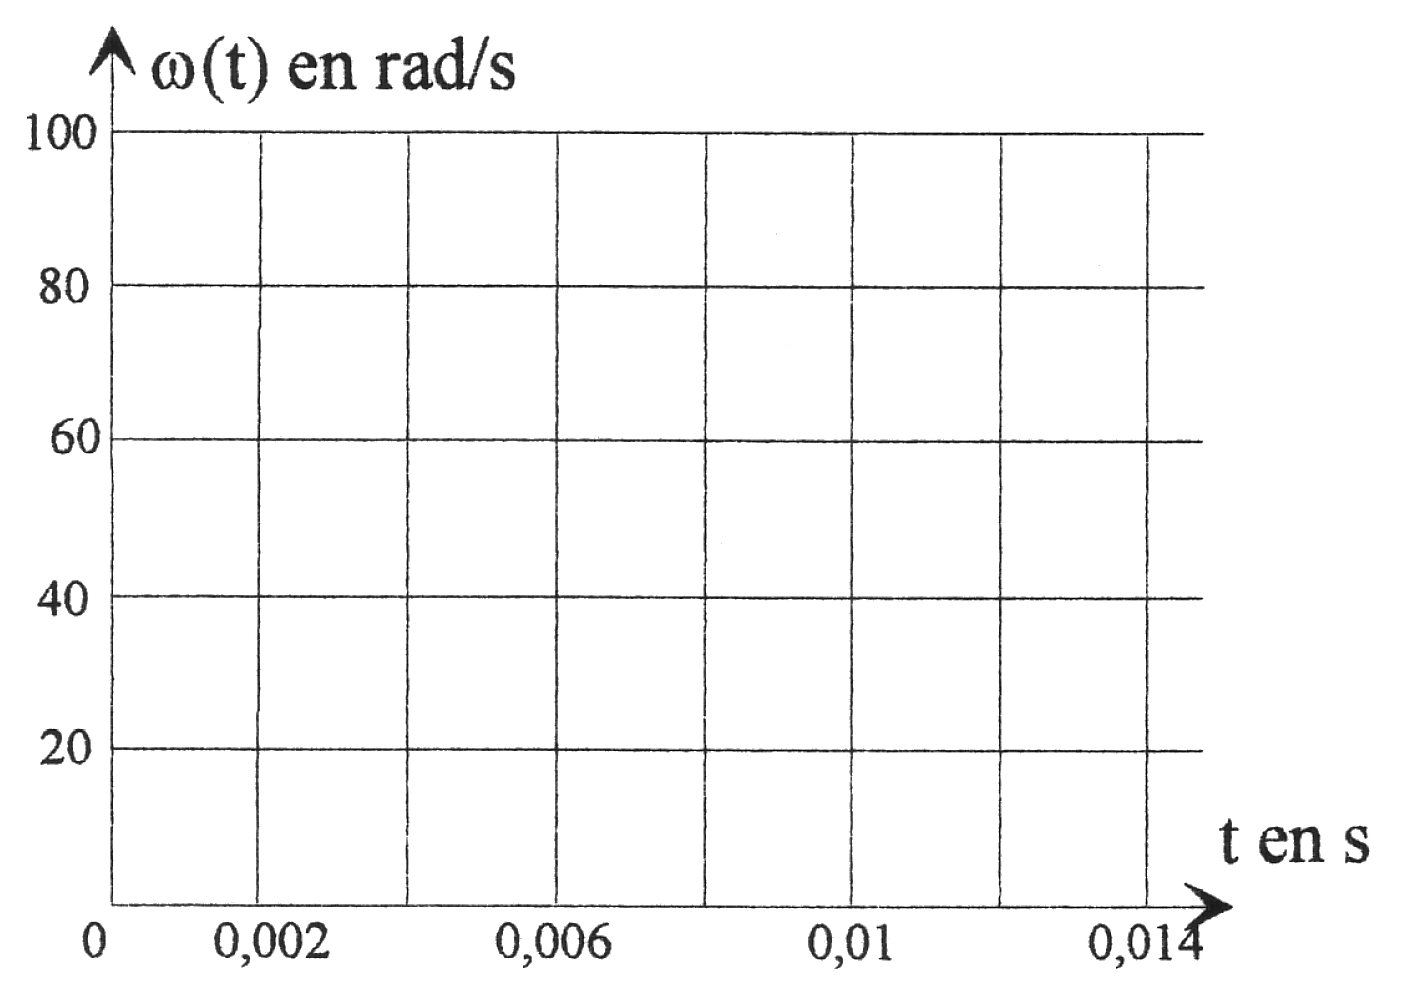
\includegraphics[width=0.7\linewidth]{img/dr06}
\end{center}}{
\begin{center}
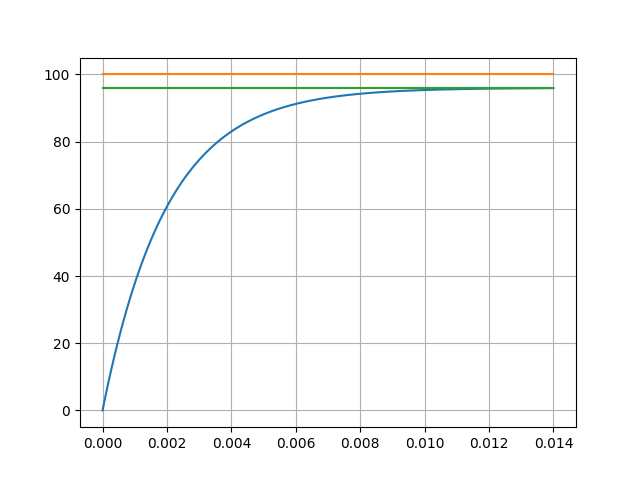
\includegraphics[width=0.7\linewidth]{img/dr06_cor}
\end{center}

Si $Ka=800$, $\tau_F=\frac{0,05}{1+0,03\cdot 800}=\frac{0,05}{25}=0,002s$

$K_F=\frac{24}{1+24}=0,96$ et $\epsilon_S=(1-0,96)\cdot 100=4rad.s^{-1}$.}

\reponse{3}{}{$\epsilon_S=2\%$, ssi $K_F=0,98=\frac{0,03\cdot Ka}{1+0,03\cdot Ka}$

$Ka=\frac{50\cdot0,98}{0,03}=1633,33$

Ainsi, $\epsilon_S\leq 2\%$ ssi $Ka\ge1633,34$}

%\newpage

\reponse{2}{}{Il y a plusieurs réponses possible pour cette question. La simplicité de la pièce fait qu'elle peut être forgée mais la faible série rend le moulage moins cher que le forgeage.}

\reponse{2}{}{A: circlips, B: clavette, C:vis}

\reponse{2}{}{La liaison 103-100 est modélisable par une rotule pour le roulement 102 et par une linéaire rectiligne pour 111.}

\reponse{2}{}{
\begin{center}
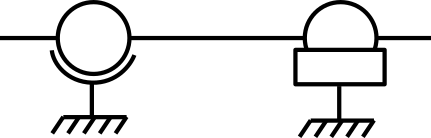
\includegraphics[width=0.5\linewidth]{img/r26}
\end{center}

La liaison globale est une liaison pivot isostatique.}

\reponse{7}{}{Pour l'ajustement 106-103,on peut choisir H7g6.}

\reponse{0}{Compléter le calque réponse}{Calque corrigé}

\reponse{0}{Compléter le calque réponse}{Calque corrigé}

\reponse{2}{}{Spécification dimensionnelle.

La distance entre deux points répartis autour du diamètre doit être comprise entre 11,8mm et 12,1mm.

Un cylindre de forme parfaite et de diamètre 11,8mm doit pouvoir passer à l'intérieur de la forme réputée cylindrique.
}

\reponse{2}{}{Élément spécifié: Axe nominalement rectiligne.

Zone de tolérance: Cylindre de diamètre 0.1mm.

Condition: L'axe nominalement rectiligne doit être compris dans la zone de tolérance.}

\reponse{2}{}{Élément spécifié: Surface nominalement plane.

Zone de tolérance: Volume compris entre deux plans parallèles distants de 0,1mm.

Condition: La surface nominalement place doit être comprise dans la zone de tolérance.}

\reponse{2}{}{Élément spécifié: Surface nominalement plane.

Référence: Surface nominalement cylindrique

Référence spécifiée: Axe du plus grand cylindre inscrit

Zone de tolérance: Volume compris entre deux plans parallèles distants de 0,3mm et perpendiculaires à A.

Condition: La surface nominalement place doit être comprise dans la zone de tolérance.}


\reponse{2}{}{Élément spécifié: Surface nominalement plane.

Référence: (A) Surface nominalement cylindrique, (B) Surface nominalement plane.

Référence spécifiée: (A) Axe du plus grand cylindre inscrit, (B) Plan perpendiculaire à A, tangent extérieur matière minimisant l'écart maximum.

Zone de tolérance: Volume compris entre deux plans parallèles distants de 0,3mm, perpendiculaires à A et dont le plan médian est situé à 9mm de B.

Condition: La surface nominalement place doit être comprise dans la zone de tolérance.}

\reponse{3}{}{$d=5\cdot N$, donc $N=\frac{32}{5}=6,4tours$}

\reponse{3}{}{
\begin{tabular}{|c|c|c|c|c|}
\hline
a-bc & 00 & 01 & 11 & 10 \\
\hline
0 & 0 & 0 & 1 & 0 \\
\hline
1 & 0 & 1 & 1 & 1 \\
\hline
\end{tabular}

On a donc $d=b.c+a.c+a.b$
}

\reponse{13}{}{\begin{center}
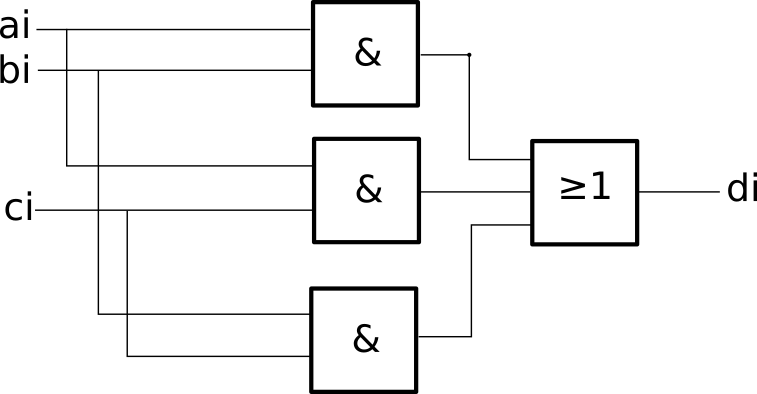
\includegraphics[width=0.5\linewidth]{img/r37}
\end{center}}

\reponse{3}{}{
\begin{tabular}{|c|c|c|c|c|}
\hline
32-10 & 00 & 01 & 11 & 10 \\
\hline
00 & 0 & 1 & 0 & 1 \\
\hline
01 & 1 & 0 & 1 & 0 \\
\hline
11 & 0 & 1 & X & X \\
\hline
10 & X & X & X & X \\
\hline
\end{tabular}

On a donc $k_0=d_0\oplus d_1\oplus d_2\oplus d_3$

\begin{tabular}{|c|c|c|c|c|}
\hline
32-10 & 00 & 01 & 11 & 10 \\
\hline
00 & 0 & 0 & 1 & 1 \\
\hline
01 & 1 & 1 & 0 & 0 \\
\hline
11 & 0 & 0 & X & X \\
\hline
10 & X & X & X & X \\
\hline
\end{tabular}

On a donc $k_1=d_1\oplus d_2\oplus d_3$

\begin{tabular}{|c|c|c|c|c|}
\hline
32-10 & 00 & 01 & 11 & 10 \\
\hline
00 & 0 & 0 & 0 & 0 \\
\hline
01 & 1 & 1 & 1 & 1 \\
\hline
11 & 0 & 0 & X & X \\
\hline
10 & X & X & X & X \\
\hline
\end{tabular}

On a donc $k_2=\overline{d_3}.d_2$

\begin{tabular}{|c|c|c|c|c|}
\hline
32-10 & 00 & 01 & 11 & 10 \\
\hline
00 & 0 & 0 & 0 & 0 \\
\hline
01 & 0 & 0 & 0 & 0 \\
\hline
11 & 1 & 1 & X & X \\
\hline
10 & X & X & X & X \\
\hline
\end{tabular}

On a donc $k_3=d_3$
}

\reponse{2}{}{}

\reponse{2}{}{$e_i=a_i.\overline{c_i}+\overline{a_i}.b_i+\overline{b_i}.c_i$}

\reponse{2}{}{\begin{center}
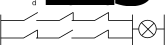
\includegraphics[width=0.5\linewidth]{img/r41}
\end{center}}

%\newpage

\ifdef{\public}{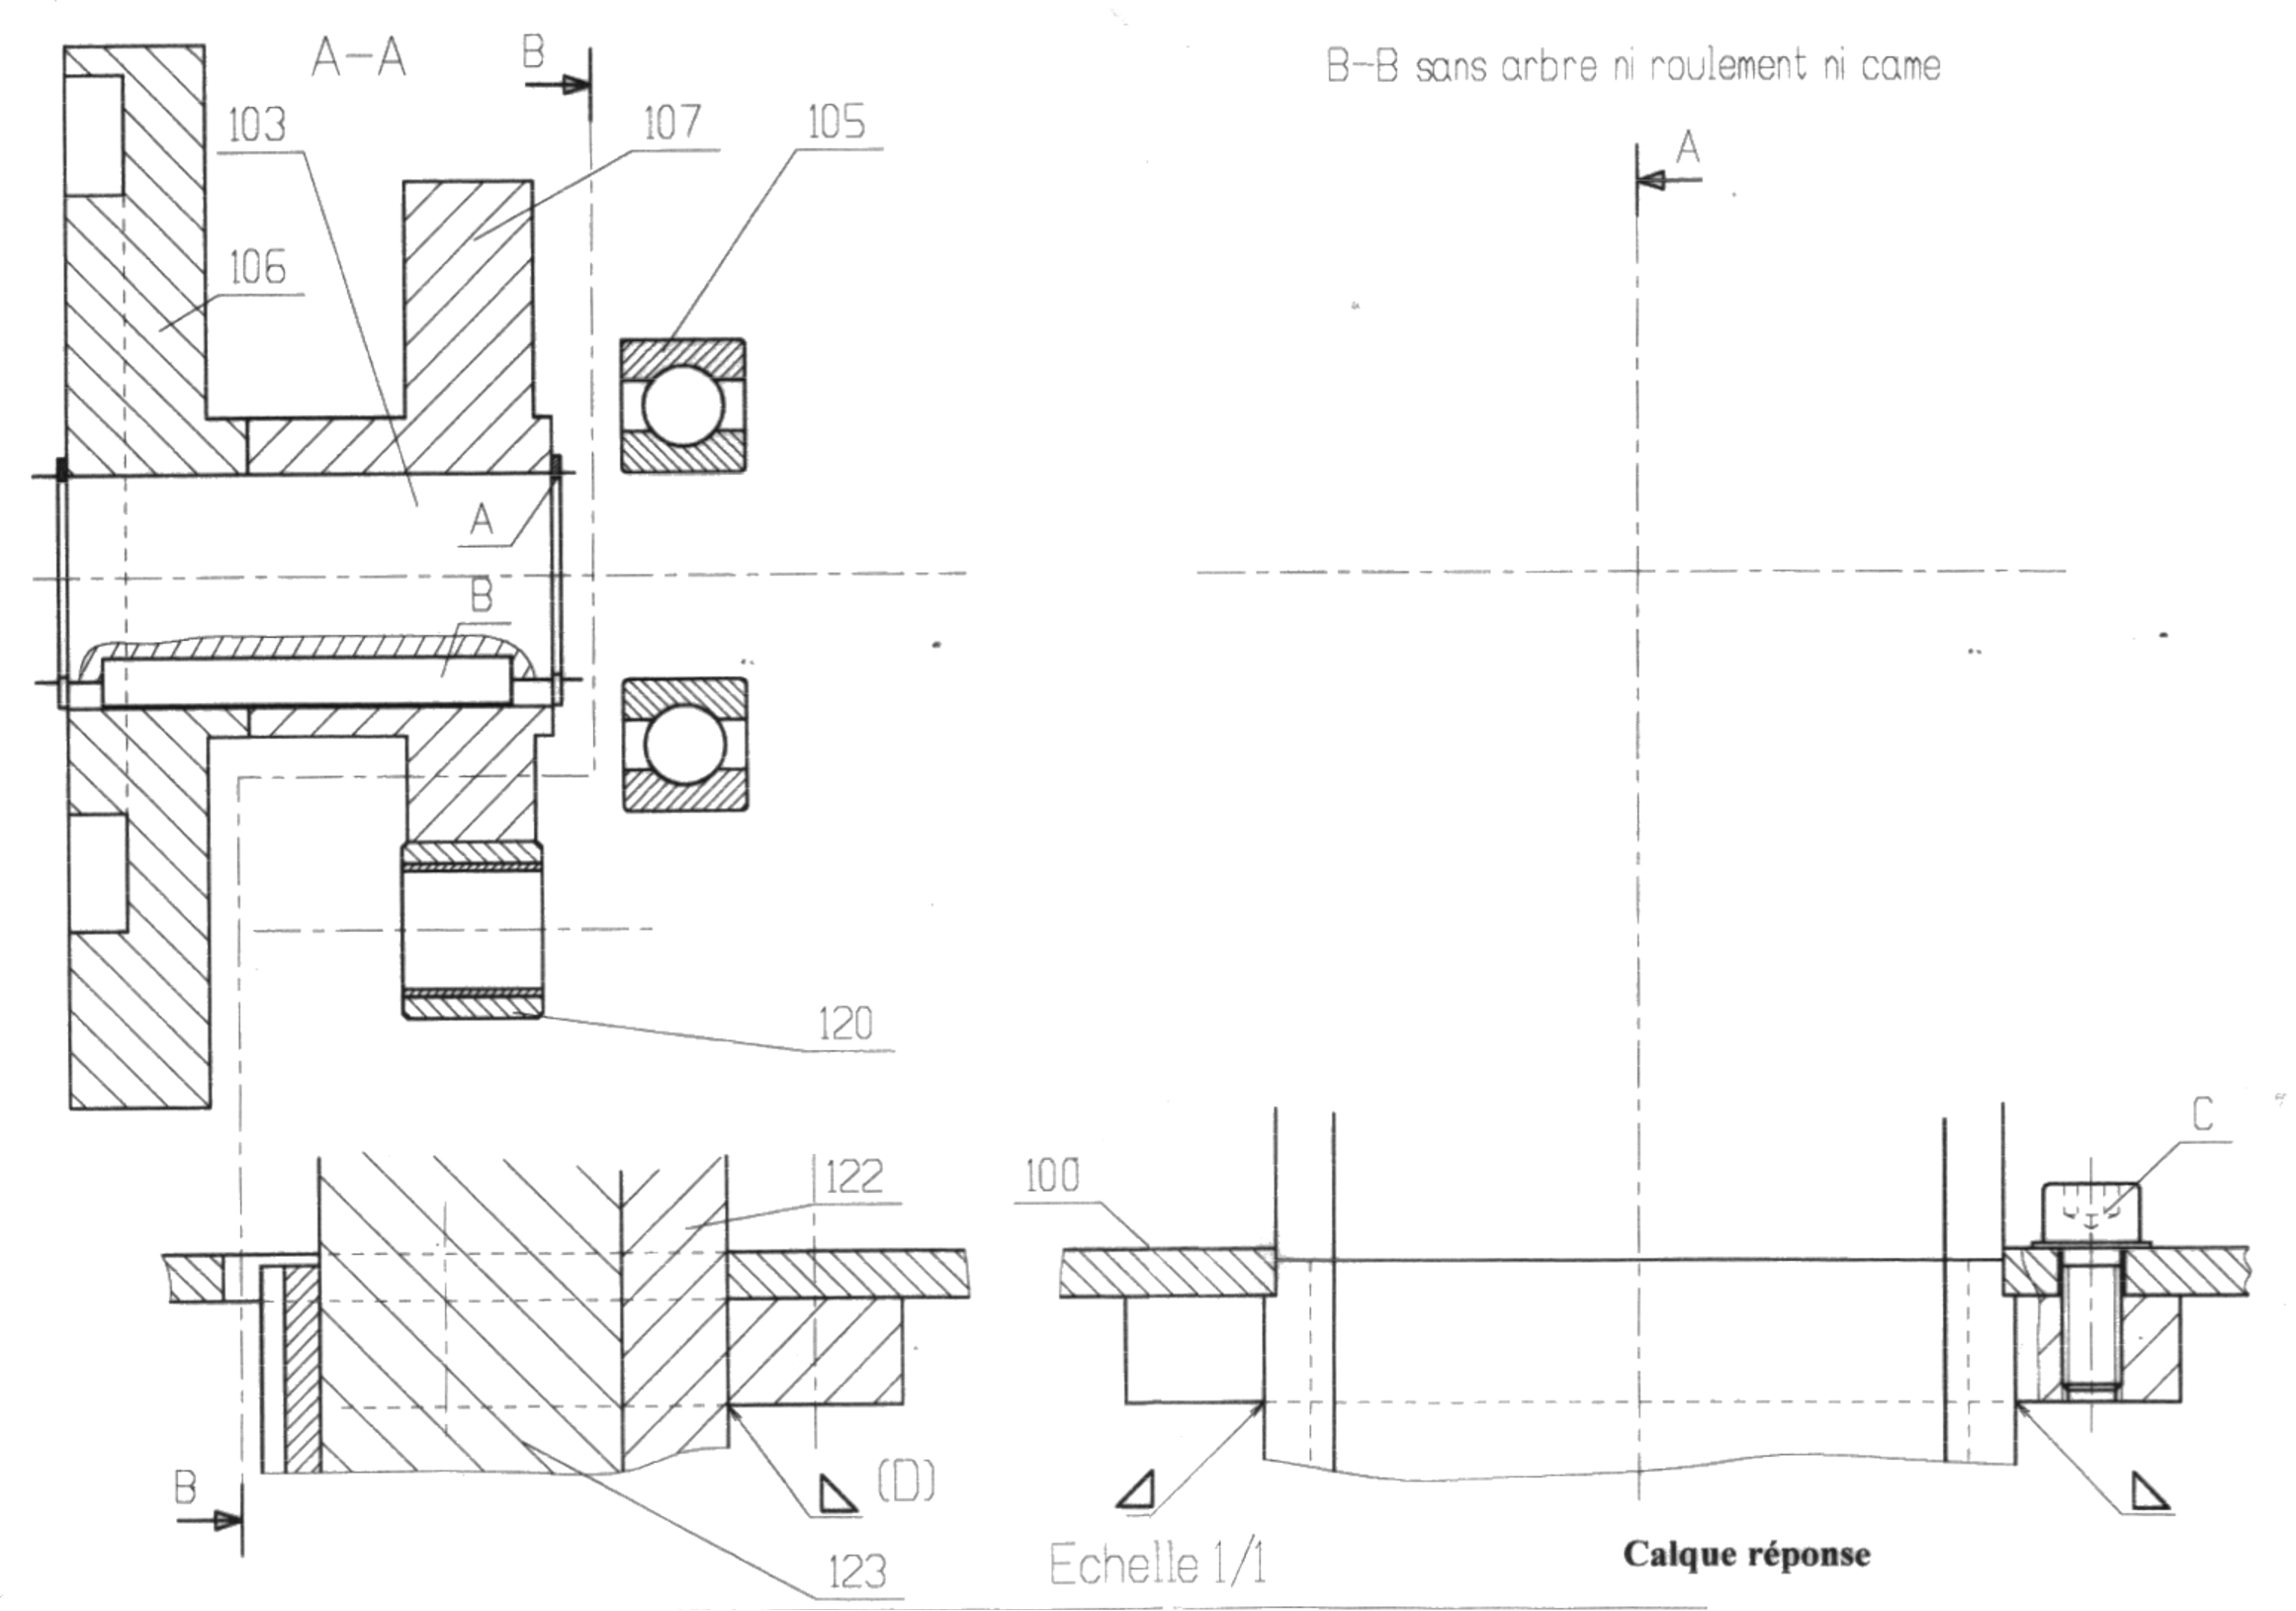
\includepdf[angle=90,offset=-0.5cm -0.5cm]{img/Calque.pdf}}
{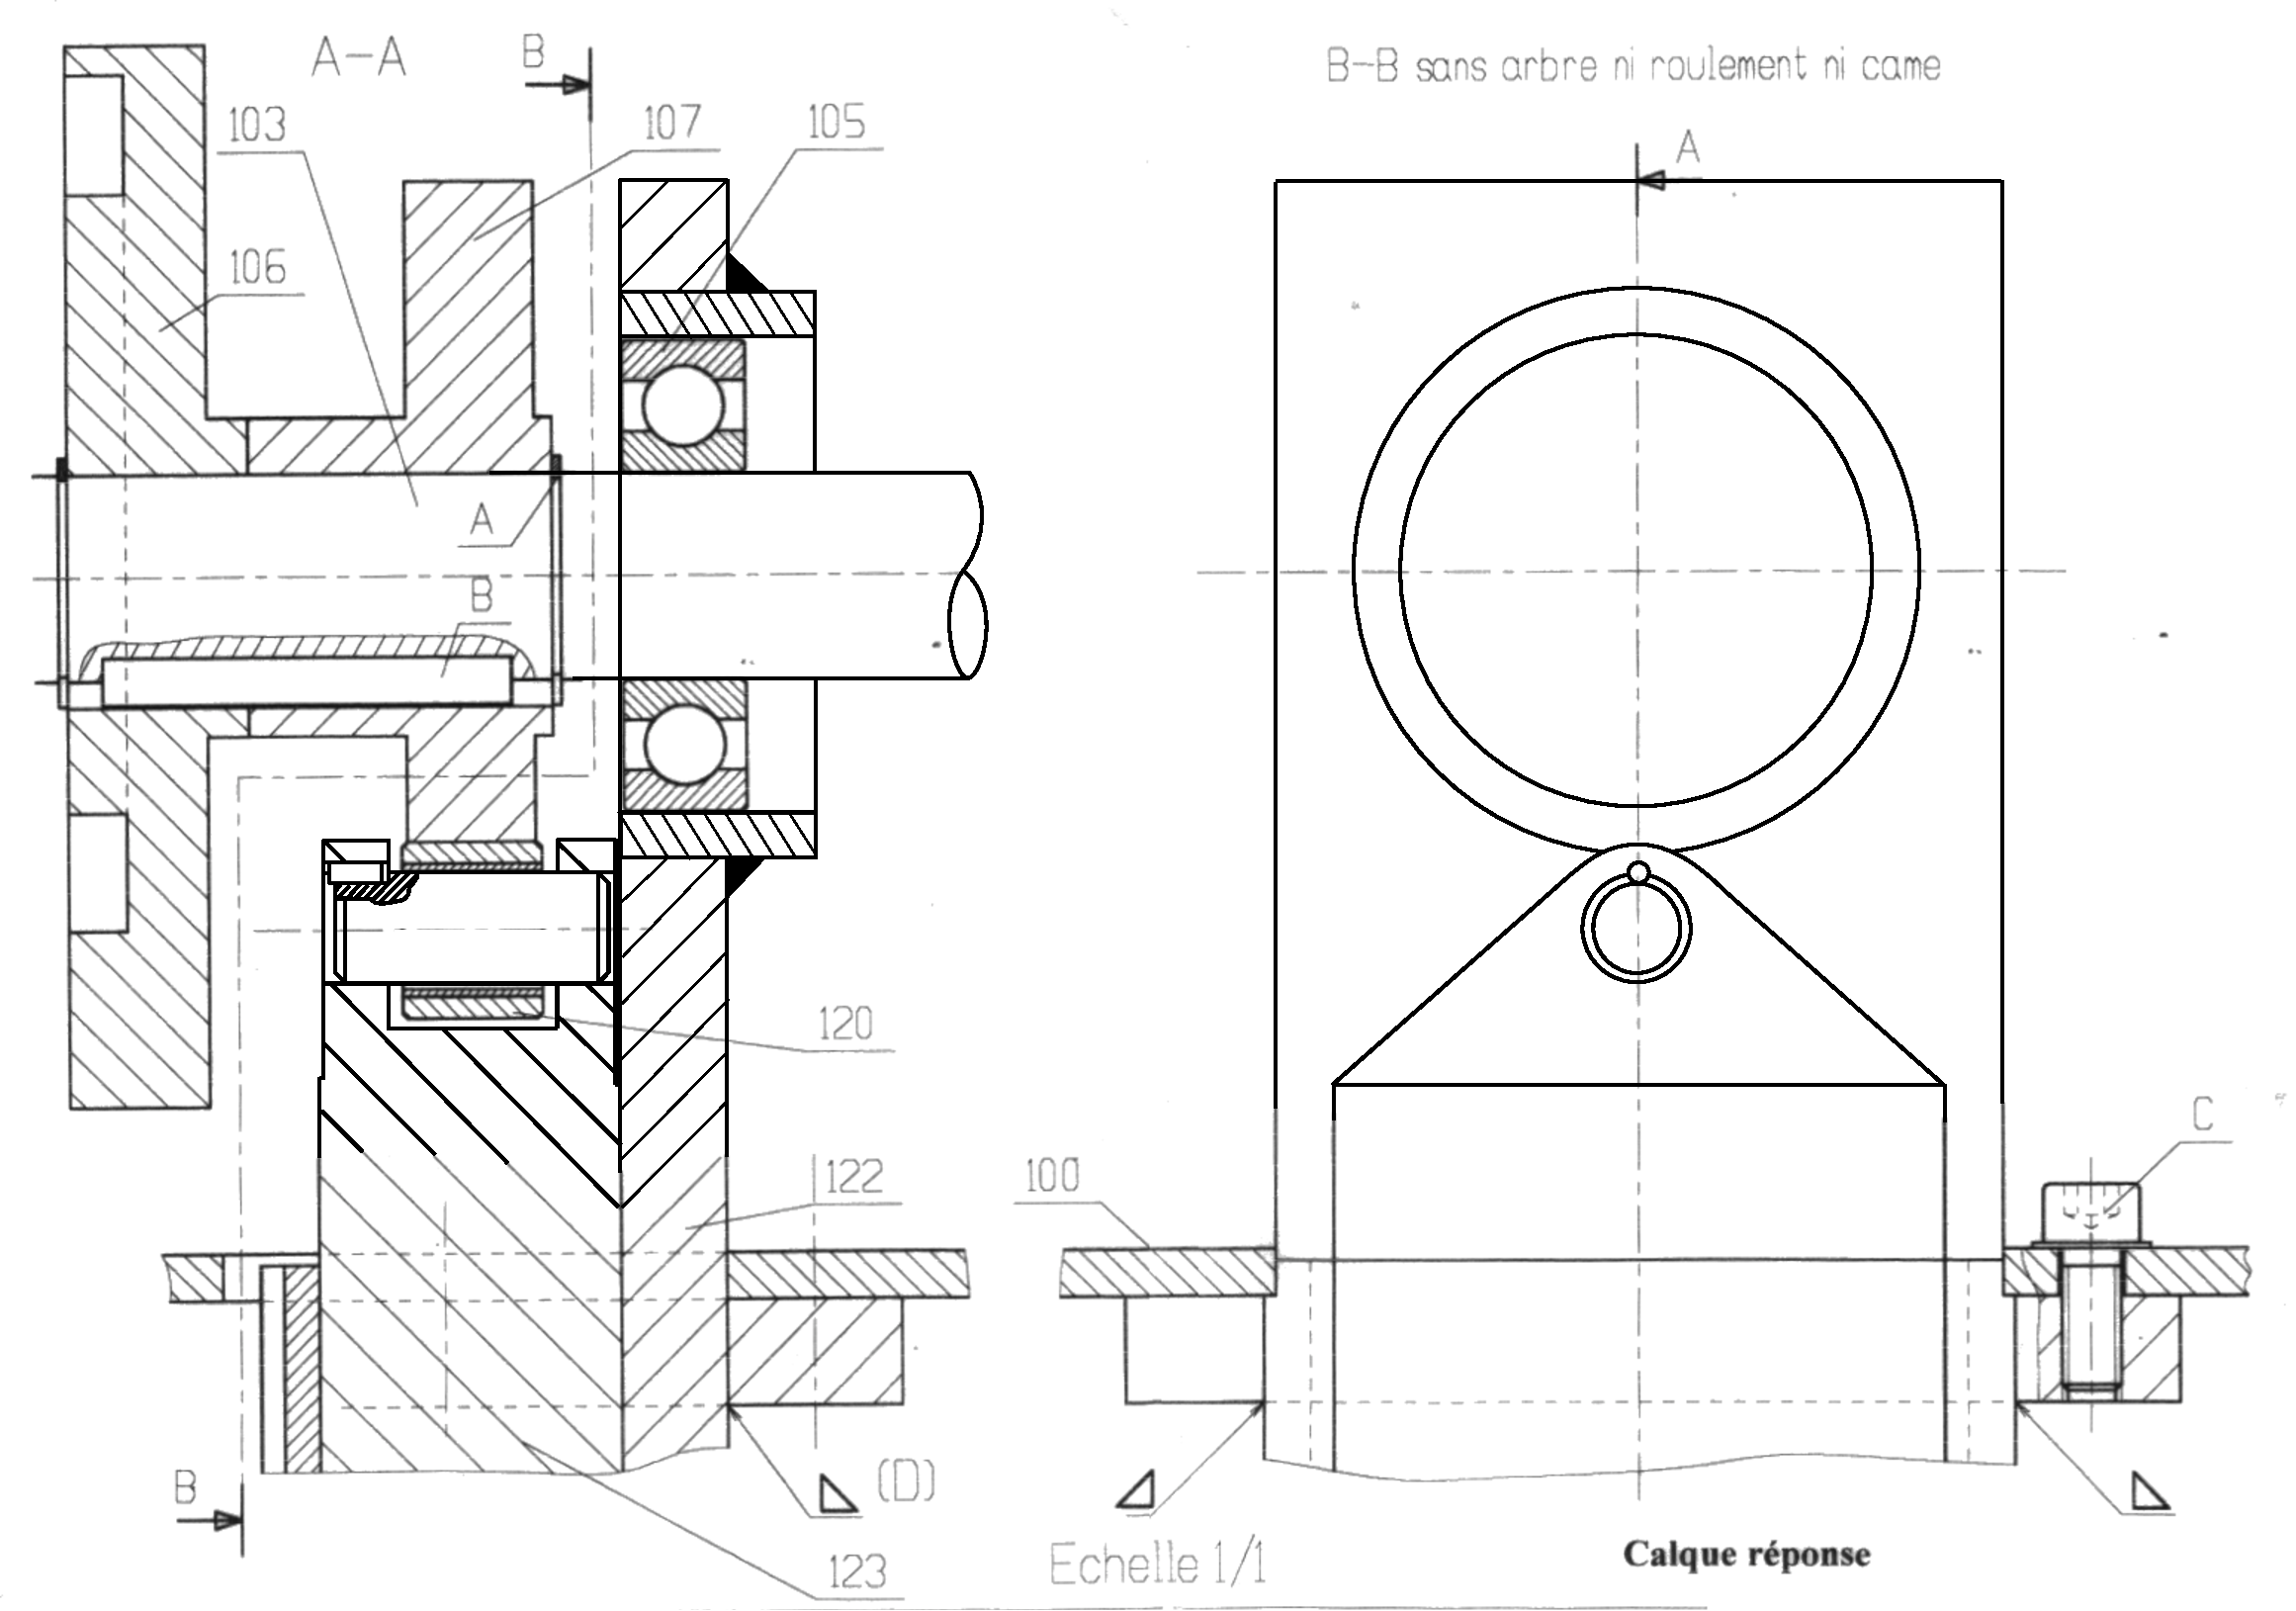
\includepdf[angle=90,offset=-0.5cm -0.5cm]{img/Calque_cor.pdf}}



\end{document}
